\documentclass[aspectratio=169]{beamer}
\usepackage[english]{babel}
\usepackage[T1]{fontenc}
\usepackage[utf8]{inputenc}
\usepackage{cite}
\usepackage{tikz}
%\usetikzlibrary{shapes,arrows,fit,calc,positioning,automata}
\usepackage{eurosym}
\usepackage{caption}
\captionsetup[figure]{labelformat=empty}

%\setbeamertemplate{navigation symbols}{}
%\usepackage{beamerthemeshadow}


\title{Development and test of FPGA firmware for the readout of the ABACUS chip for beam monitoring applications in hadron therapy}
\author[Stefan Zugravel]{Candidate: \\ Stefan Cristi Zugravel \\ --------------------------------- \\ Supervisor: \\ Prof. Luca Pacher\\ ---------------------------------  \\ Co-Supervisor: \\ Prof. Vincenzo Monaco}
\date{\today}
\institute[UniTo]{University of Turin}
\logo{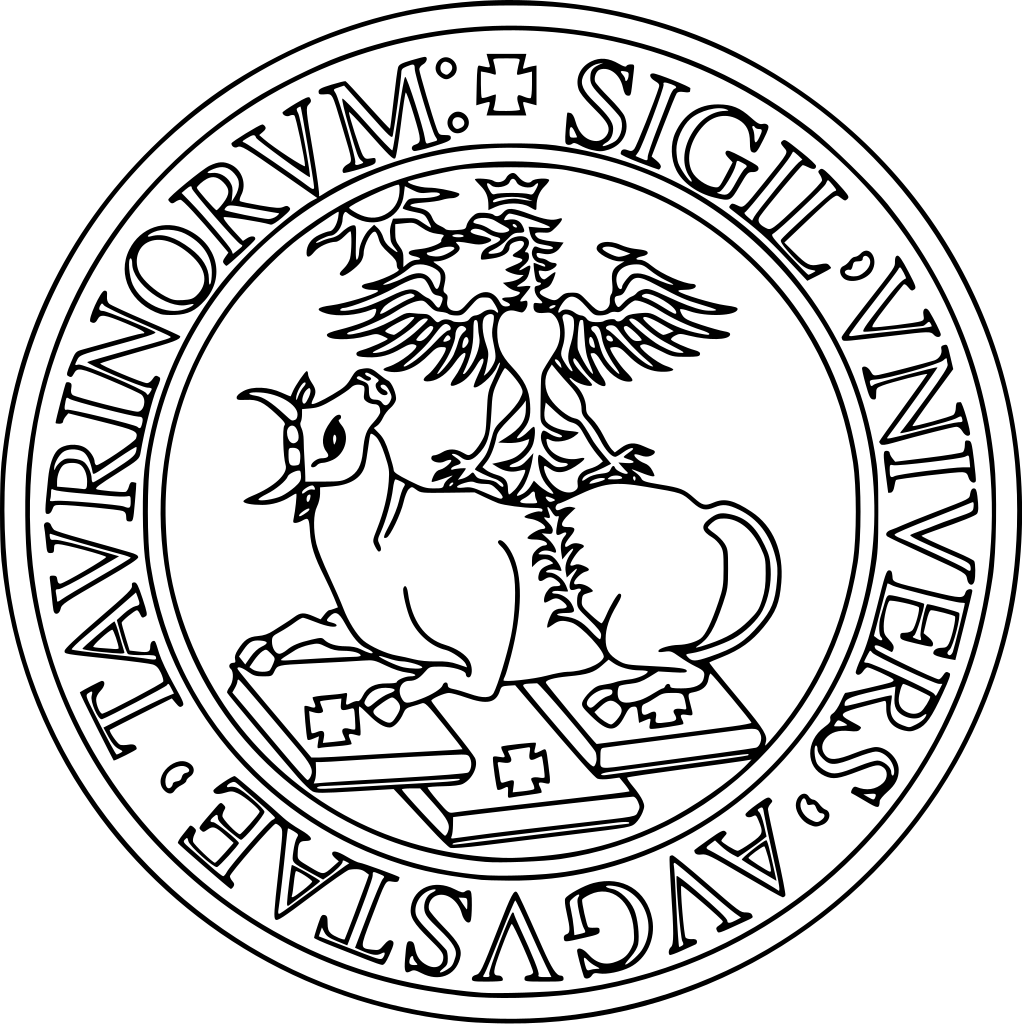
\includegraphics[width=10mm]{IMG/Unito.png}}
%\usetheme{Antibes}
\usetheme{Madrid}
%\setbeamercovered{dynamic}
\setbeamertemplate{footline}[frame number]
%\beamertemplatenavigationsymbolsempty
\setbeamertemplate{navigation symbols}{}
\begin{document}
	
	\begin{frame}		
		\maketitle
	\end{frame}

	\begin{frame}
	\frametitle{Table of contents}
		\begin{columns}
			\column{0.3 \textwidth}
				\begin{center}
					\tableofcontents
				\end{center}
			\column{0.7 \textwidth}
				\begin{center}
					
\includegraphics[width=0.95 \textwidth]{IMG/Move_IT_logo.PNG}
				\end{center}
		\end{columns}
	\vspace{1 cm}
	\begin{itemize}
		\item MoVe\_IT = \textbf{Mo}deling and \textbf{Ve}rification for \textbf{I}on beam \textbf{T}reatment planning
	\end{itemize}
	\end{frame}

%%%%%%%%%%%%%%%%%%%%%%%%%%%%%%%%%%%%%%%%%%%%%%%%%%%%%%%%%%%%%%%%%%%%%%%%%%%%%%%%%%%%%%%%
	\section{Hadron therapy}
	
	\begin{frame}
	\frametitle{Hadron therapy, sensor and ASICs}
	\begin{center}
		{\Huge \fontfamily{qtm}\selectfont \color{blue} \textbf{Hadron therapy, sensor and ASICs}}
	\end{center}
\end{frame}
	
	\begin{frame}
	\frametitle{Hadron therapy}
	\begin{columns}
		\column{0.40 \textwidth}
		\begin{center}
			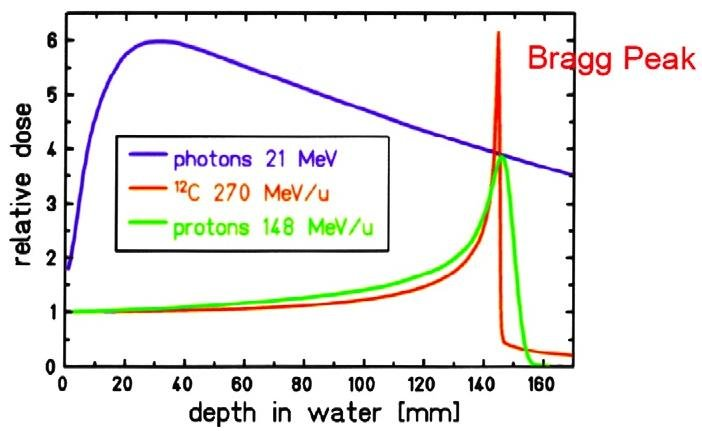
\includegraphics[width=0.75 \textwidth]{IMG/Bragg_Peak.PNG}
			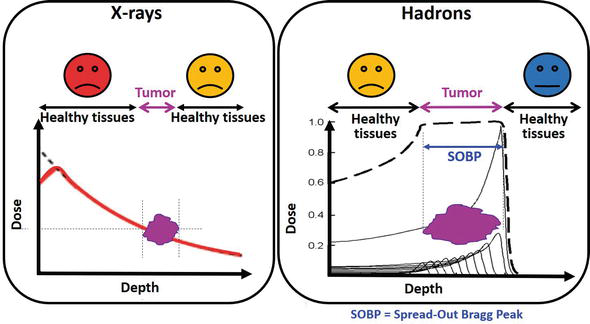
\includegraphics[width=0.65 \textwidth]{IMG/Bragg_Peak2.PNG}
		\end{center}
		\column{0.60 \textwidth}
		\begin{center}
			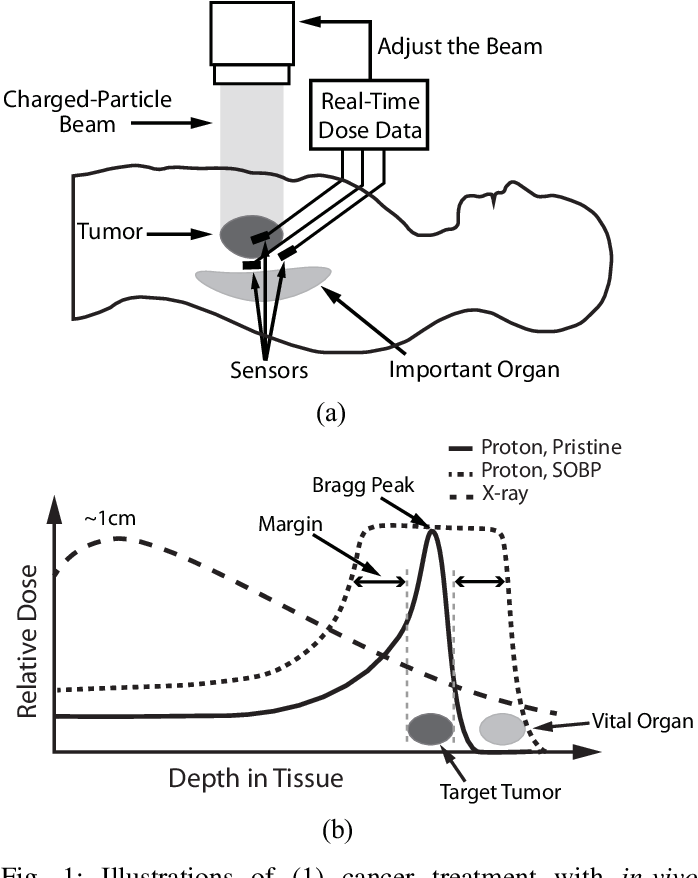
\includegraphics[width=0.3 \textwidth]{IMG/HadroTherapy.PNG}
			\newline
			Typical particle rate for a therapeutical beam is :
			\begin{itemize}
				\item $10^6 \:- \: 10^8 \: \frac{cm^2}{s}$ for carbon ions
				\item $10^8 \:- \: 10^{10} \: \frac{cm^2}{s}$ for protons
			\end{itemize}
		\end{center}
	\end{columns}
	\begin{center}
		\begin{equation}
			-\dfrac{\mathrm dE}{\mathrm dx} = 2 \pi N_{a} r_{e}^{2} m_{e} c^{2} \rho \dfrac{Z}{A}  \dfrac{z^{2}}{\beta^{2}}\left[\ln\left(\dfrac{2m_{e} \gamma ^{2} v^{2} W_{max}}{I^{2}}\right) - 2\beta^{2} - \delta 2\frac{C}{Z}\right]
		\end{equation}
	\end{center}
	
	\end{frame}

%%%%%%%%%%%%%%%%%%%%%%%%%%%%%%%%%%%%%%%%%%%%%%%%%%%%%%%%%%%%%%%%%%%%%%%%%%%%%%%%%%%%%%%%
	\section{LGAD sensors}
	
	\begin{frame}
	\frametitle{LGAD sensors}
		\begin{center}
			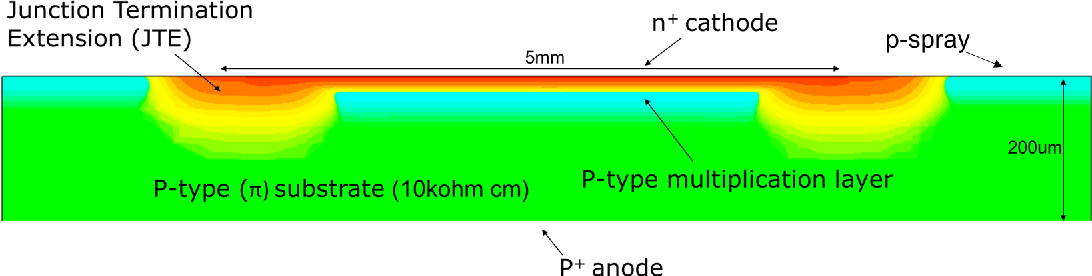
\includegraphics[width=0.9 \textwidth]{IMG/LGAD_image.PNG}
		\end{center}
	\textbf{L}ow \textbf{G}ain \textbf{A}valanche \textbf{D}etectors
		\begin{itemize}
			\item 1-1.5cm long strips with 200$\mu$m pitch
			\item 50$\mu$m sensor thickness
			\item Internal gain of \textbf{10-15} 
			\item Trapezoidal signal of $\approx$\textbf{1.2ns}
		\end{itemize}
	\end{frame}

%%%%%%%%%%%%%%%%%%%%%%%%%%%%%%%%%%%%%%%%%%%%%%%%%%%%%%%%%%%%%%%%%%%%%%%%%%%%%%%%%%%%%%%%
	\section{ABACUS2 ASIC}
	

	\begin{frame}
	\frametitle{ABACUS2-1}
		\begin{columns}
			\column{0.5 \textwidth}
			\begin{center}
				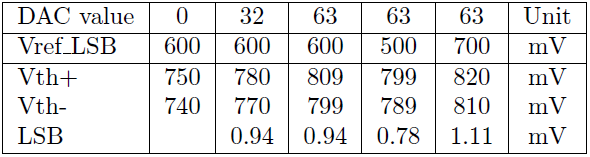
\includegraphics[width=0.8 \textwidth]{IMG/TableLSB.PNG}
				\newline
				The threshold can be fine-tuned at the channel level with a \textbf{6-bits} DAC. The DACs can linearly increase the threshold with a nominal LSB value of \textbf{0.94mV}. The LSB value can be tuned via the Vref LSB input.
			\end{center}
			\begin{itemize}
				\item \textbf{24} channels
				\item UMC \textbf{110nm} technology
				\item Die size 4.95 x 1.935 mm$^2$
				\item Internal Dacs \textbf{1.2V single ended} serial signal
			\end{itemize}
			\column{0.5 \textwidth}
			\begin{itemize}
				\item Initialization sequence \textbf{A5A5}= 
				\newline
				1010-0101-1010-0101
				\item \textbf{16bit words} 2bit command + 6bit address + 8bit data
				\begin{itemize}
					\item \textbf{command}
					\begin{itemize}
						\item \textbf{11} = write
						\item \textbf{10} = read
					\end{itemize}
					\item \textbf{address}
					\begin{itemize}
						\item \textbf{5bit} address from \textbf{0} to \textbf{23}
						\item \textbf{LSB} is Vth+- (not used for now)
					\end{itemize}
					\item \textbf{data}
					\begin{itemize}
						\item \textbf{2MSB} not used
						\item \textbf{6LSB} data for the internal DAC \newline from \textbf{0} to \textbf{63}
					\end{itemize}
				\end{itemize} 
			\end{itemize}
		\end{columns}
	\end{frame}

	
	\begin{frame}
	\frametitle{ABACUS2-2}
	\begin{center}
		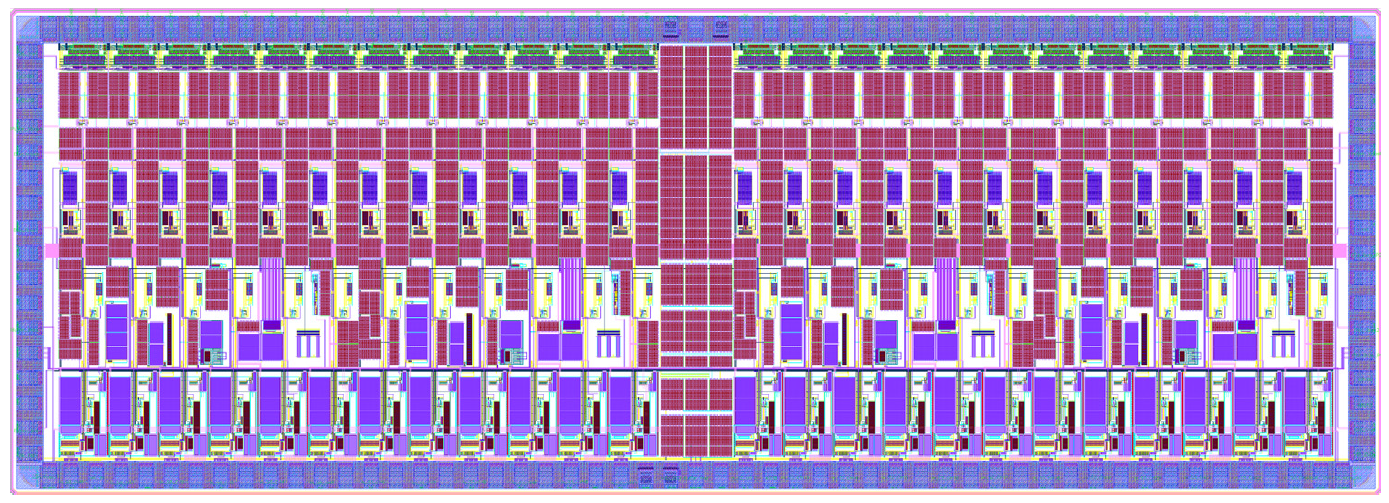
\includegraphics[width=0.6 \textwidth]{IMG/ABACUS.PNG}
		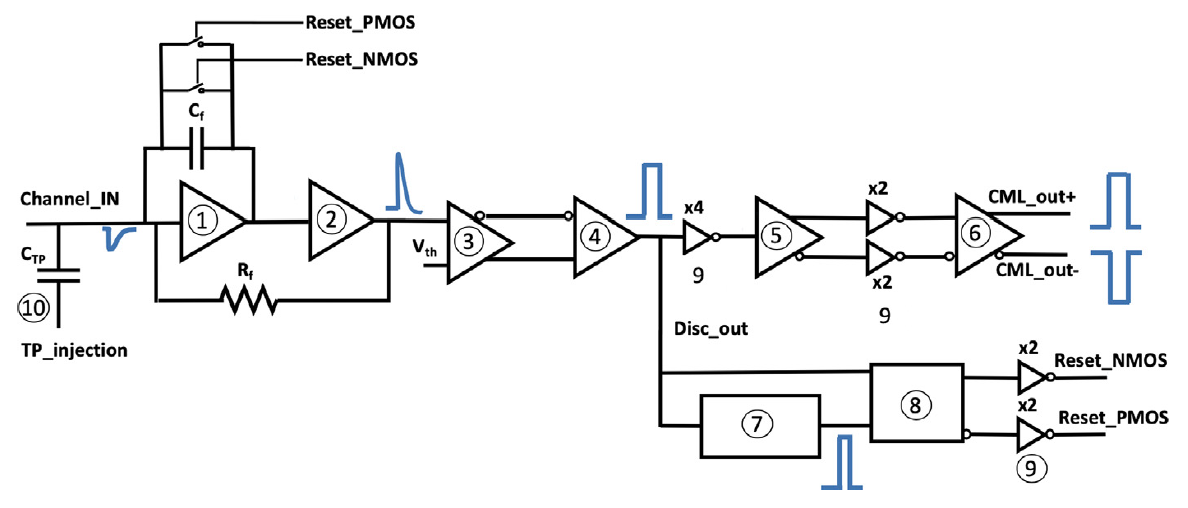
\includegraphics[width=0.6 \textwidth]{IMG/ABACUS_channel.PNG}
	\end{center}
	\end{frame}

%%%%%%%%%%%%%%%%%%%%%%%%%%%%%%%%%%%%%%%%%%%%%%%%%%%%%%%%%%%%%%%%%%%%%%%%%%%%%%%%%%%%%%%%
	\section{FPGA}
	
		
	\begin{frame}
	\frametitle{FPGA \& VHDL}
	\begin{center}
		{\Huge \fontfamily{qtm}\selectfont \color{blue} \textbf{FPGA \& VHDL}}
	\end{center}
	\end{frame}
	
	\begin{frame}
	\frametitle{FPGA}
	{\Large 
		\begin{itemize}
			\item FPGA = \textbf{F}ield \textbf{P}rogrammable \textbf{G}ate \textbf{A}rray
			\begin{itemize}
				\item gate array : \textbf{array of "logic cells"} that can be programmed to implement \textbf{any desired logic functionality}
				\item field programmable: \textbf{device not committed to do something} until effectively programmed according to the field application
			\end{itemize}
		\item in principle, \textbf{programmable infinite times} with no limitations
		\item \textbf{high flexibility}: it can be implemented \textbf{any digital function}
		\item \textbf{fast} and \textbf{cheap} prototyping cycle
		\begin{itemize}
			\item \textbf{out of the box} solution: no layout, masks or other manufacturing steps needed
		\end{itemize}
		\item {\color{orange} power hungry, slow compared to \textbf{ASICs} and expensive on large-scales}
		\end{itemize}
	}
	\end{frame}

	\begin{frame}
	\frametitle{FPGA}
	\begin{columns}
		\column{0.5 \textwidth}
		\begin{center}
			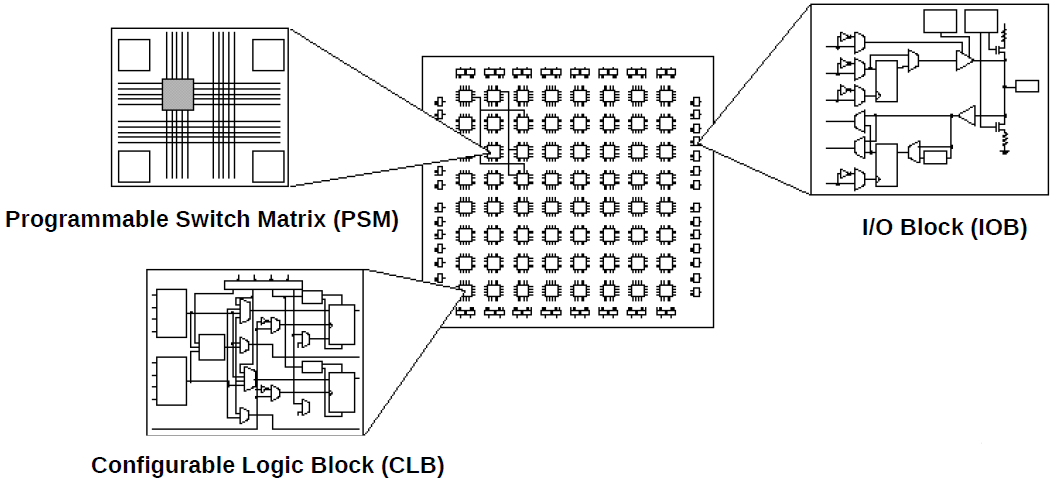
\includegraphics[width=0.75 \textwidth]{IMG/FPGA_PARTS.PNG}
			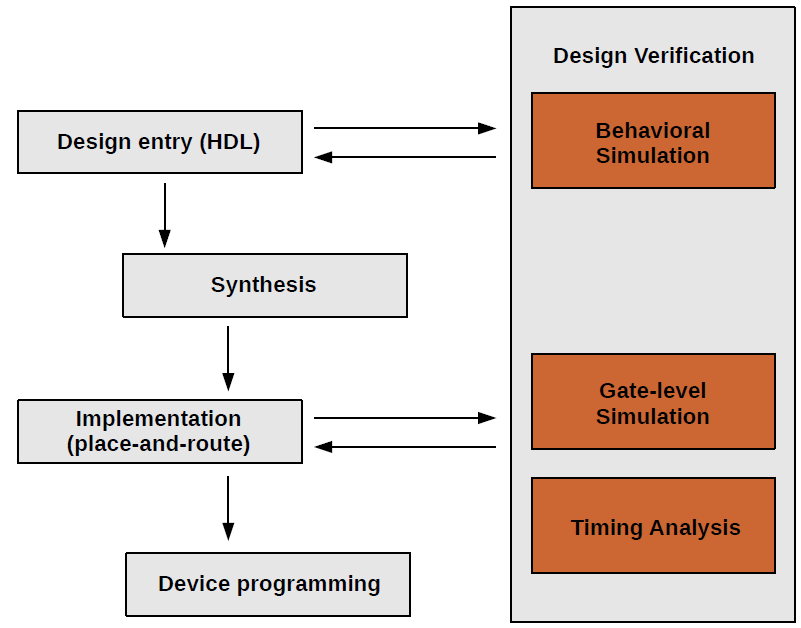
\includegraphics[width=0.65 \textwidth]{IMG/DesignFlow.PNG}
		\end{center}
		\column{0.5 \textwidth}
		\begin{itemize}
			\item \textbf{PSM}: \textbf{P}rogrammable \textbf{S}witch \textbf{M}atrix = Whenever a vertical and a horizontal channel intersect, there is a switch box. When a wire enters a switch box there are programmable switches that allow it to connect to other wires in adjacent channel segments
			\item \textbf{IOB}: \textbf{I}/\textbf{O} \textbf{B}lock = collection or grouping of basic elements that implement the input and output functions of an FPGA device
			\item \textbf{CLB}: \textbf{C}onfigurable \textbf{L}ogic \textbf{B}lock = A typical cell consists of a 4-input LUT, a Full adder (FA) and a D-type flip-flop
		\end{itemize}
	\end{columns}
	\end{frame}

	
	\begin{frame}
	\frametitle{FPGA board }
	\begin{center}
		\textbf{Kintex7 kc705 board}
		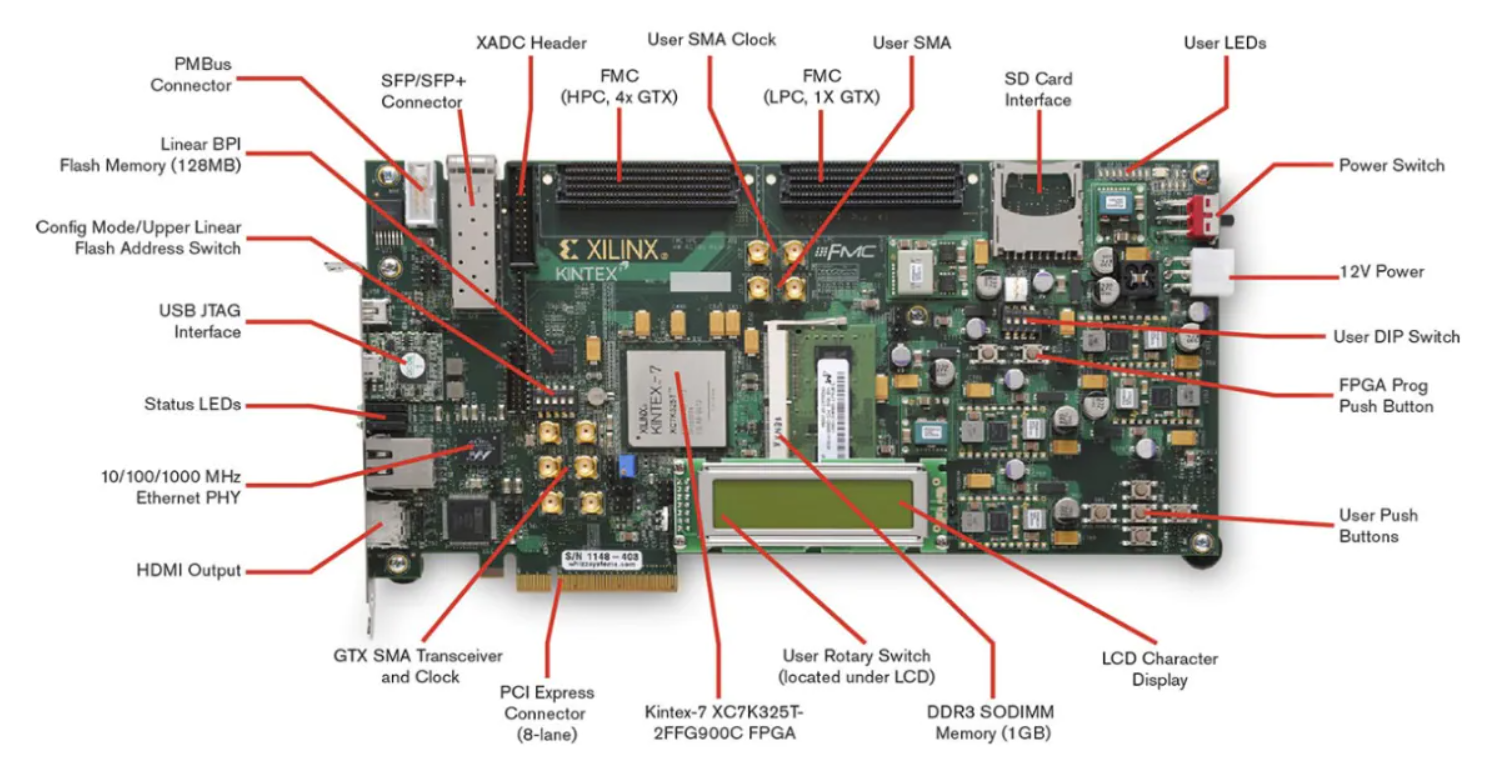
\includegraphics[width=0.85 \textwidth]{IMG/KC705.PNG}
	\end{center}
	\end{frame}

	\begin{frame}
	\frametitle{VHDL}
	{\LARGE
	\begin{itemize}
		\item \textbf{VHDL}: \textbf{V}HSIC \textbf{H}ardware \textbf{D}escription \textbf{L}anguage 
		\begin{itemize}
			\item \textbf{VHSIC}: \textbf{V}ery \textbf{H}igh \textbf{S}peed \textbf{I}ntegrated \textbf{C}ircuits
			\item is a hardware description language (\textbf{HDL}) that can model the behavior and structure of digital systems at multiple levels of abstraction
			\item since \textbf{1987}, VHDL has been standardized by the Institute of Electrical and Electronics Engineers (\textbf{IEEE})
			\item in February 2008, Accellera approved \textbf{VHDL 4.0}, also informally known as VHDL 2008
			\item {\color{orange} VHDL is not a programming language!}
		\end{itemize}
	\end{itemize}
	}
	\end{frame}


	\begin{frame}
	\frametitle{Test bench, Test board and Debug Tool}
	\begin{center}
		{\Huge \fontfamily{qtm}\selectfont \color{blue} \textbf{Test bench, Test board and Debug Tool}}
	\end{center}
	\end{frame}


	\begin{frame}
	\frametitle{Test bench}
	\begin{center}
		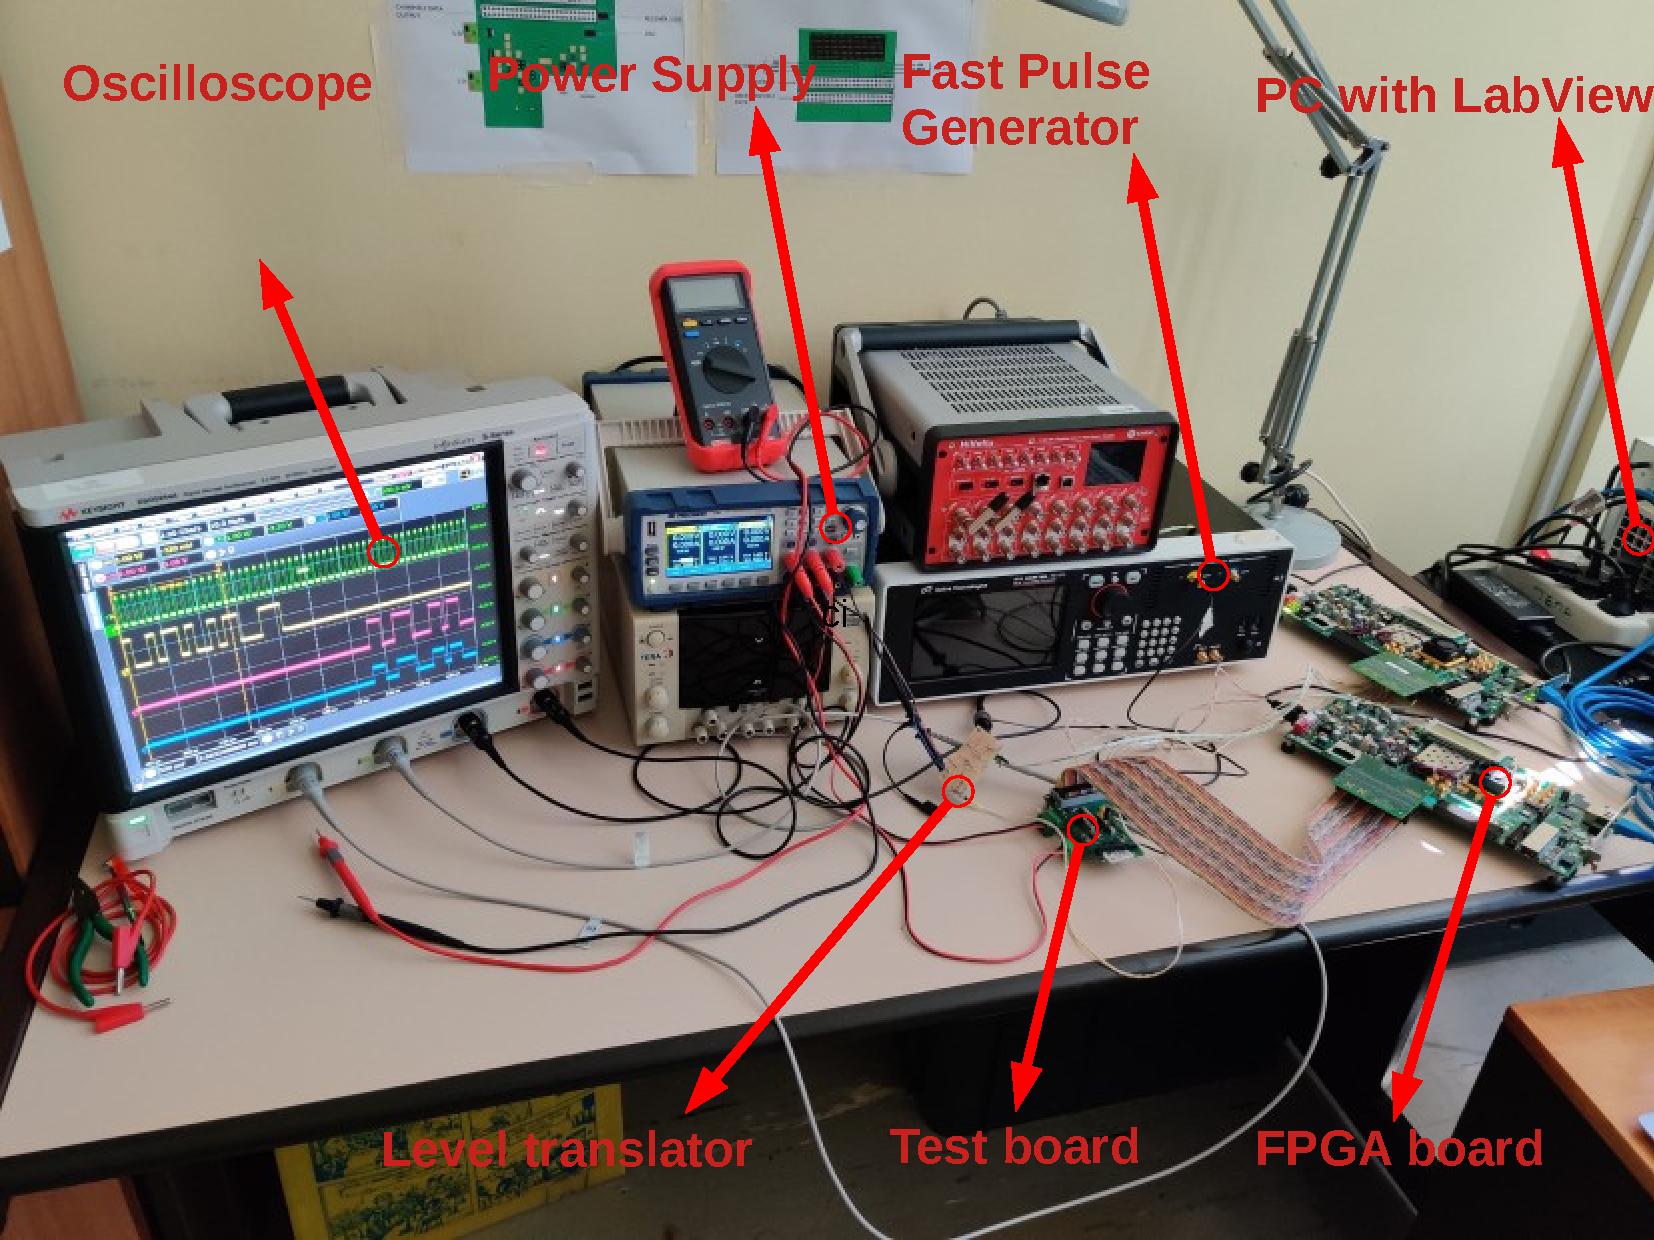
\includegraphics[width=0.65 \textwidth]{IMG/TestBench.pdf}
	\end{center}
	\end{frame}

	\begin{frame}
	\frametitle{Test board}
	\begin{itemize}
		\item 3.3V power supply
		\item 1 ABACUS ASIC chip
		\item Resistive voltage divider to translate signal amplitude
	\end{itemize}
	\begin{center}
		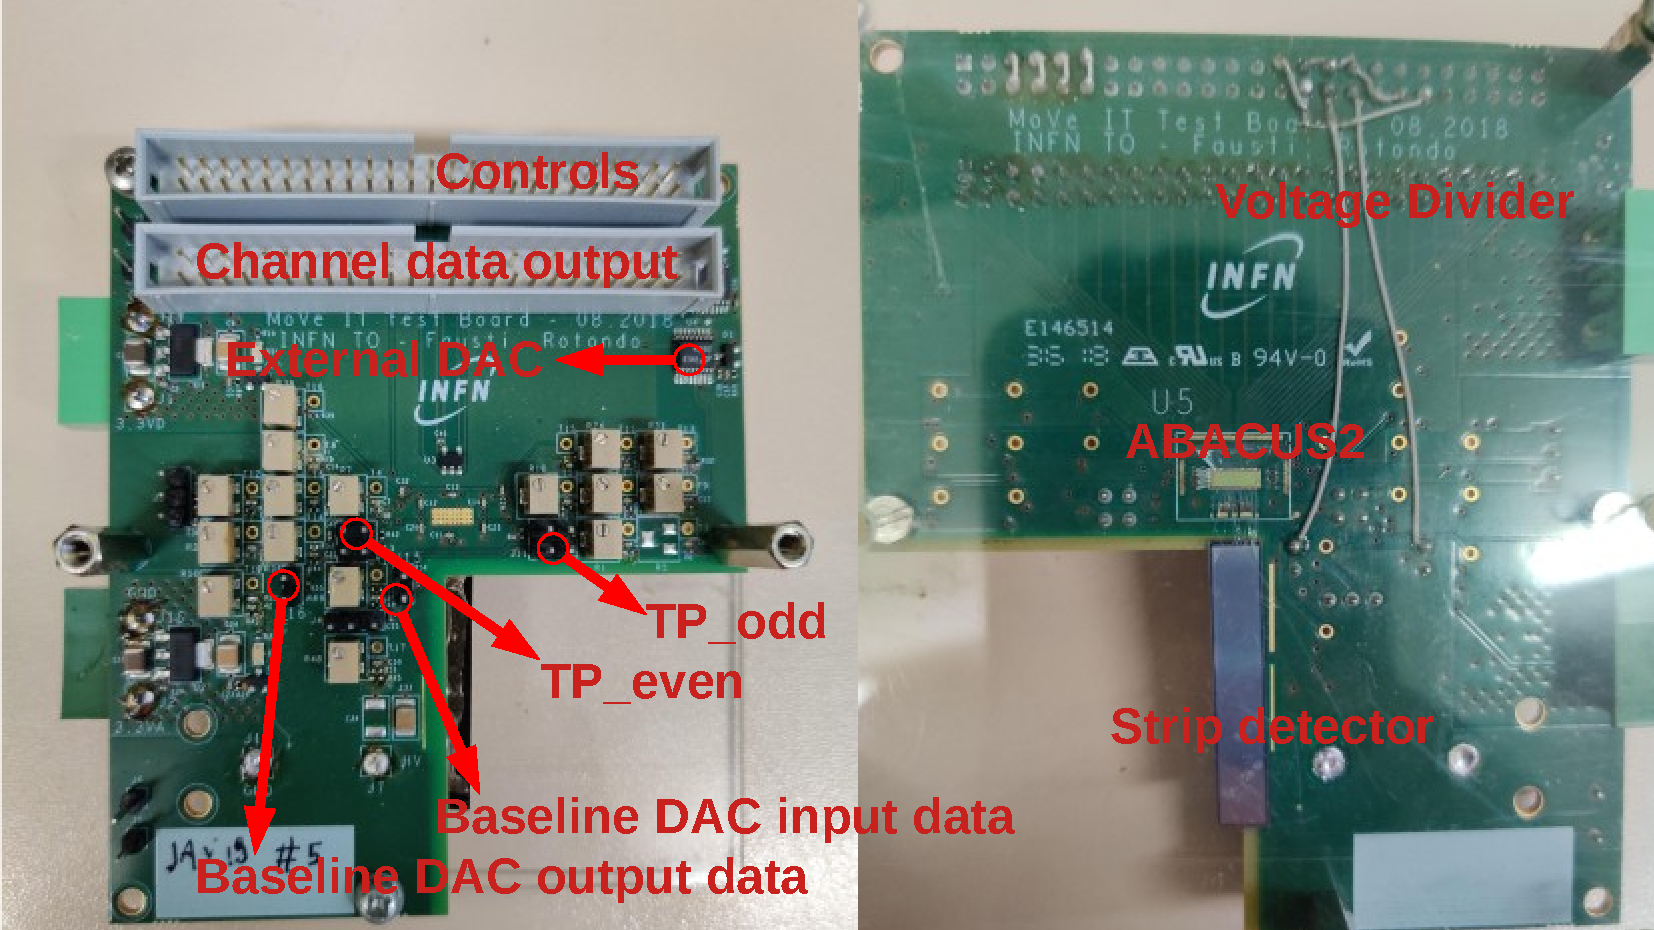
\includegraphics[width=0.7 \textwidth]{IMG/TestBoard.pdf}
	\end{center}
	\end{frame}

	\begin{frame}
	\frametitle{LabView Software}
	\begin{itemize}
		\item LabView software written by Emanuele Data
		\item write or read one channel at the time
		\item write or read all 24 channels
	\end{itemize}
	\begin{center}
		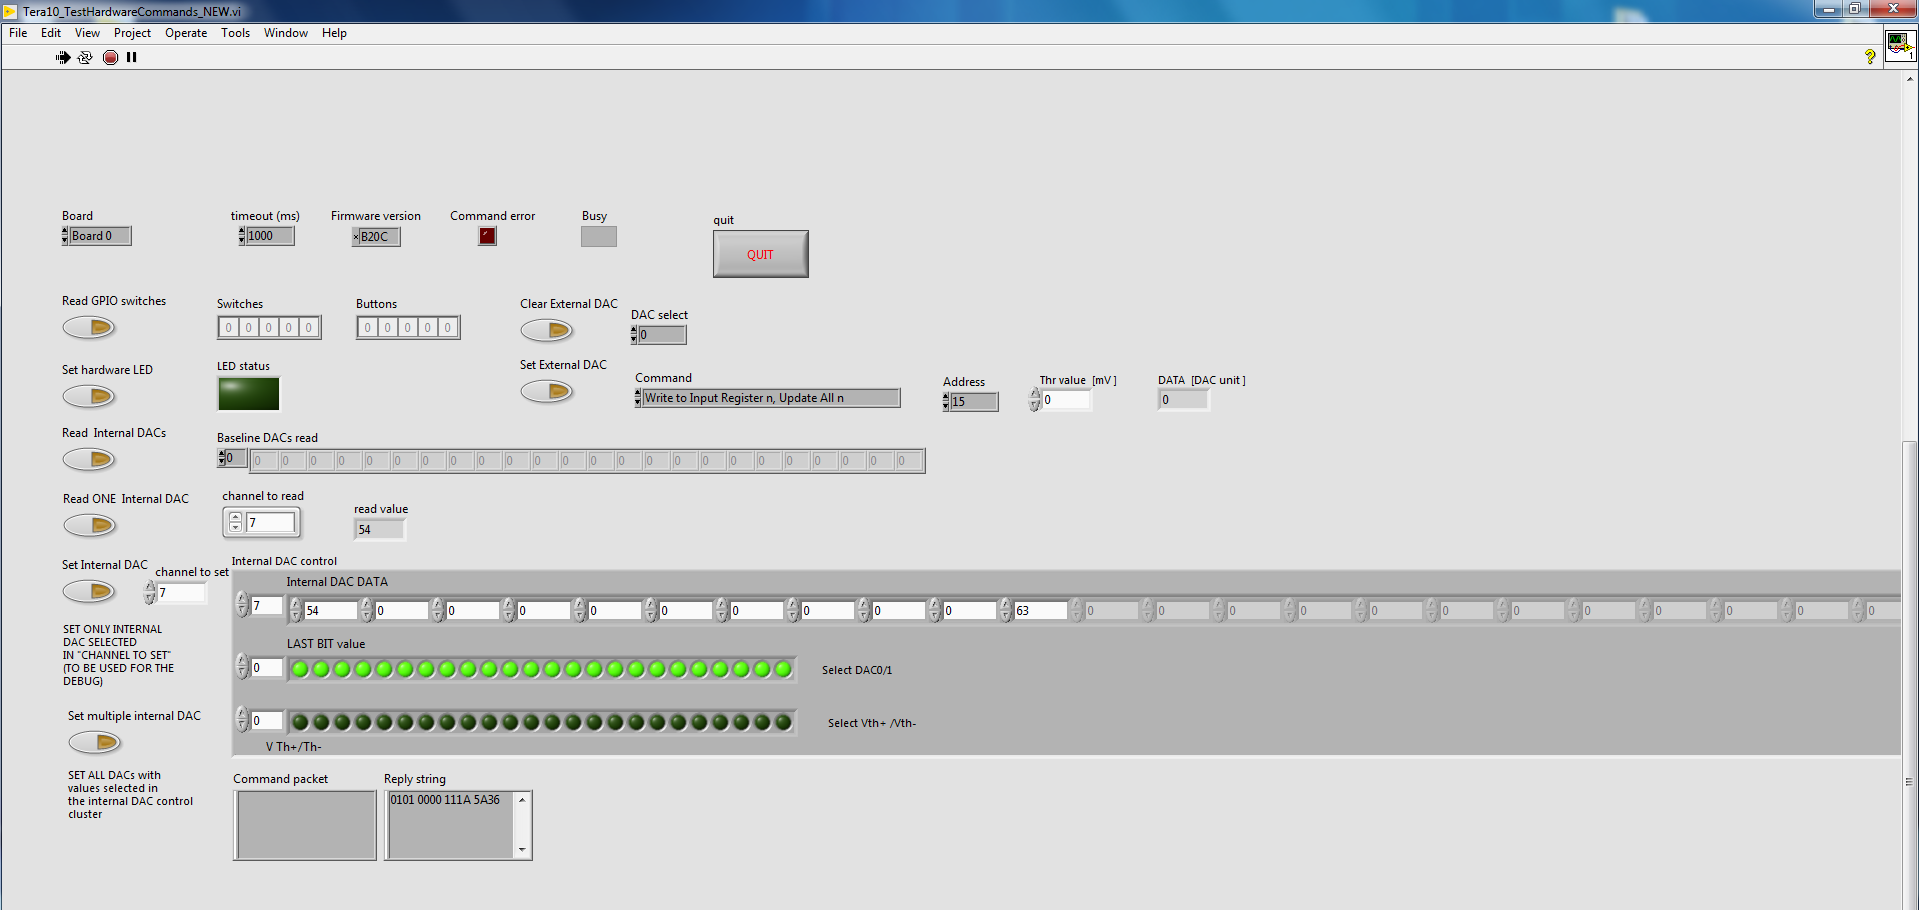
\includegraphics[width=0.7 \textwidth]{IMG/LabVIEWBaselineDac.PNG}
	\end{center}
	\end{frame}

	
%%%%%%%%%%%%%%%%%%%%%%%%%%%%%%%%%%%%%%%%%%%%%%%%%%%%%%%%%%%%%%%%%%%%%%%%%%%%%%%%%%%%%%%%
	\section{Firmware}
	
	
	
	\begin{frame}[fragile]
	\frametitle{Debug Tool}
	\begin{itemize}
		\item Debug tool to verify the working condition of every \textbf{FMC}(\textbf{HPC}/\textbf{LPC}) output
	\end{itemize}
	\begin{center}
		{\small \color{blue} Step1: Signal names and identification.}
	\end{center}
	{\tiny
		\begin{verbatim}
			pin68				: out std_logic;--H4  FMC_HPC_CLK0_M2C_P    LVDS D27         -P3 + v
			pin69				: out std_logic;--H5  FMC_HPC_CLK0_M2C_N    LVDS C27         -P4 - v 
		\end{verbatim} }
	\begin{center}
		{\small \color{blue} Step2: Differential Signalling output buffer.}
	\end{center}
	{\tiny
		\begin{verbatim}
		attribute IOSTANDARD of pin68_OBUFDS : label is "LVDS_25";	
		pin68_OBUFDS : unisim.vcomponents.OBUFDS
		port map (
		I		=> pin68_int,
		O		=> pin68,
		OB		=> pin69);		
		\end{verbatim} }
	\begin{center}
		{\small \color{blue} Step3: Constraints settings.}
	\end{center}
	{\tiny
		\begin{verbatim}
		# FMC_HPC_CLK0_M2C_P
		# FMC_HPC_CLK0_M2C_N
		set_property -dict { PACKAGE_PIN D27	IOSTANDARD LVDS_25 DIFF_TERM TRUE }	[get_ports pin68]
		set_property -dict { PACKAGE_PIN C27	IOSTANDARD LVDS_25 DIFF_TERM TRUE }	[get_ports pin69]
		\end{verbatim} }
	\end{frame}

	\begin{frame}
	\frametitle{Firmware and waveforms}
	\begin{center}
		{\Huge \fontfamily{qtm}\selectfont \color{blue} \textbf{Firmware and Waveforms}}
	\end{center}
	\end{frame}


	\begin{frame}[fragile]
	\frametitle{Writing Baseline DACs $\rightarrow$ code}
	\begin{itemize}
		\item the \textbf{FPGA} communicates with the pc using UDP (\textbf{U}ser \textbf{D}atagram \textbf{P}rotocol) implemented in the \textbf{GBphy} project
		\item each UDP packet is \textbf{64} bit long $\rightarrow$ \textbf{32} bit used by GBphy and \textbf{32} bit of data
		\item \textbf{32} bit data =
		\begin{itemize}
			\item \textbf{4} bit $\rightarrow$ firmware target
			\item \textbf{8} bit $\rightarrow$ firmware command
			\item \textbf{20} bit $\rightarrow$ firmware data
		\end{itemize}
		\item \textbf{20} bit firmware data =
		\begin{itemize}
			\item \textbf{3} bit not used
			\item \textbf{2} bit baseline dac command
			\item \textbf{6} bit baseline dac address
			\item \textbf{8} bit baseline dac data
			\item \textbf{1} bit baseline dac selecet (each FPGA can control 2 chips)
		\end{itemize}
		\item To perform a Read/write operation the initialization sequence must be sent first\newline every time
	\end{itemize}
	\end{frame}

	\begin{frame}[fragile]
		\frametitle{Writing Baseline DACs $\rightarrow$ code}
		\begin{itemize}
			\item FSM (\textbf{F}inite \textbf{S}tate \textbf{M}achine): states for the serial data communication
		\end{itemize}
		{\tiny
		\begin{columns}
		\column{0.5 \textwidth}
		
		\begin{center}
			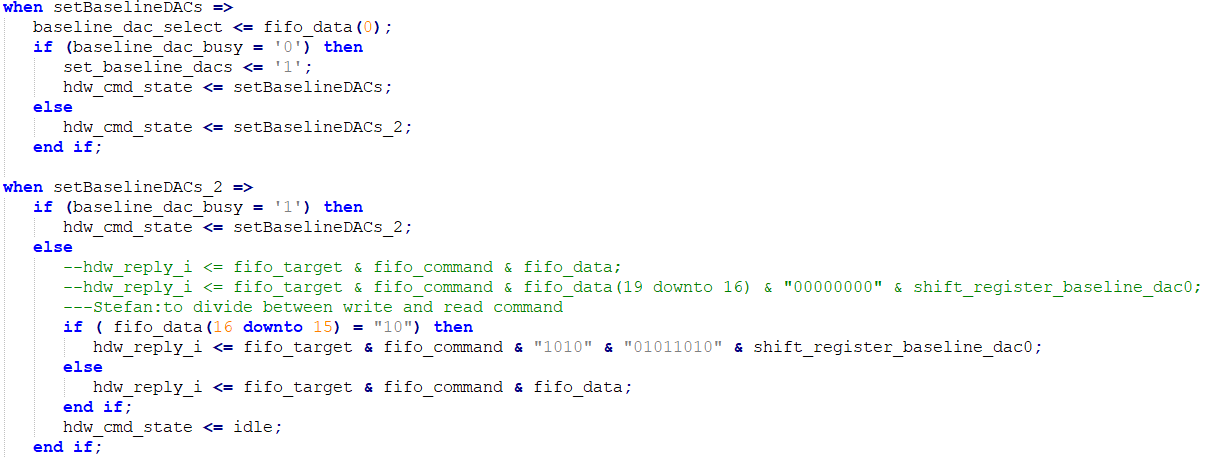
\includegraphics[width=0.95 \textwidth]{IMG/SetbaselineDac.png}
			
			\vspace{1 cm}
			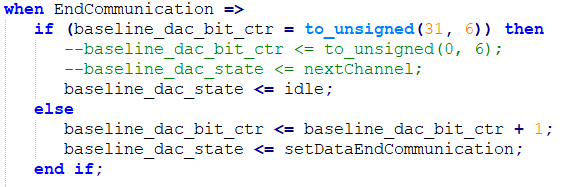
\includegraphics[width=0.85 \textwidth]{IMG/EndCommunication.png}
		\end{center}
		
	
		\column{0.5 \textwidth}
		\begin{center}
			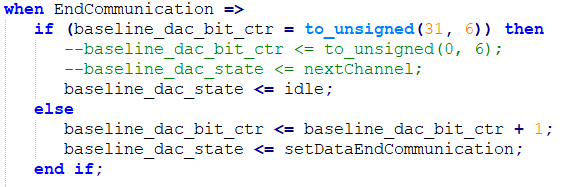
\includegraphics[width=0.85 \textwidth]{IMG/EndCommunication.png}
			
			\vspace{1 cm}
			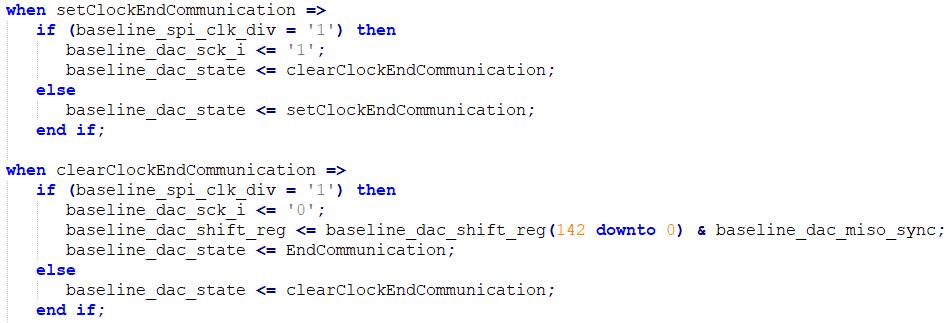
\includegraphics[width=0.85 \textwidth]{IMG/EndCommunication2.png}
		\end{center}
	
		\end{columns}
	}
	\end{frame}

	\begin{frame}[fragile]
	\frametitle{Writing Baseline DACs $\rightarrow$ code}
	\begin{itemize}
		\item FSM: \textbf{setData} state
	\end{itemize}
	{\tiny
		\begin{columns}
			\column{0.1 \textwidth}		
			
			\column{0.4 \textwidth}
			\begin{center}
				\begin{verbatim}
				when setData =>
				if (baseline_spi_clk_div = '1') then
				case baseline_dac_bit_ctr is
				when "000000" =>
				baseline_dac_mosi_i <= '1';
				when "000001" =>
				baseline_dac_mosi_i <= '0';
				when "000010" =>
				baseline_dac_mosi_i <= '1';
				when "000011" => 
				baseline_dac_mosi_i <= '0';		
				when "000100" =>
				baseline_dac_mosi_i <= '0';
				when "000101" =>
				baseline_dac_mosi_i <= '1';
				when "000110" =>
				baseline_dac_mosi_i <= '0';
				when "000111" =>
				baseline_dac_mosi_i <= '1';		
				when "001000" =>
				baseline_dac_mosi_i <= '1';
				when "001001" =>
				baseline_dac_mosi_i <= '0';
				when "001010" =>
				baseline_dac_mosi_i <= '1';
				          .
				          .
				          .
				\end{verbatim}
			\end{center}
			
			\column{0.4 \textwidth}
			\begin{center}
				\begin{verbatim}
				--command
				when "010000" =>
				baseline_dac_mosi_i <= fifo_data(16); 
				when "010001" =>
				baseline_dac_mosi_i <= fifo_data(15); 
				--address
				when "010010" =>
				baseline_dac_mosi_i <= fifo_data(14); 
				when "010011" =>
				baseline_dac_mosi_i <= fifo_data(13); 
				when "010100" =>
				baseline_dac_mosi_i <= fifo_data(12); 
				when "010101" =>
				baseline_dac_mosi_i <= fifo_data(11); 
				when "010110" =>
				baseline_dac_mosi_i <= fifo_data(10); 
				when "010111" =>
				baseline_dac_mosi_i <= fifo_data(9);  
				--data
				when "011000" =>
				baseline_dac_mosi_i <= fifo_data(8);  
				when "011001" =>
				baseline_dac_mosi_i <= fifo_data(7);  
				when "011010" =>
				baseline_dac_mosi_i <= fifo_data(6);  
				          .
				          .
				          .
				\end{verbatim}
			\end{center}
		\column{0.1 \textwidth}
		\end{columns} 
	}
	\end{frame}

	\begin{frame}
	\frametitle{Vivado simulation}
	\begin{itemize}
		\item In order to reduce the simulation time the clock was reduced to $\approx1.5\mu s$
	\end{itemize}
		\begin{center}
			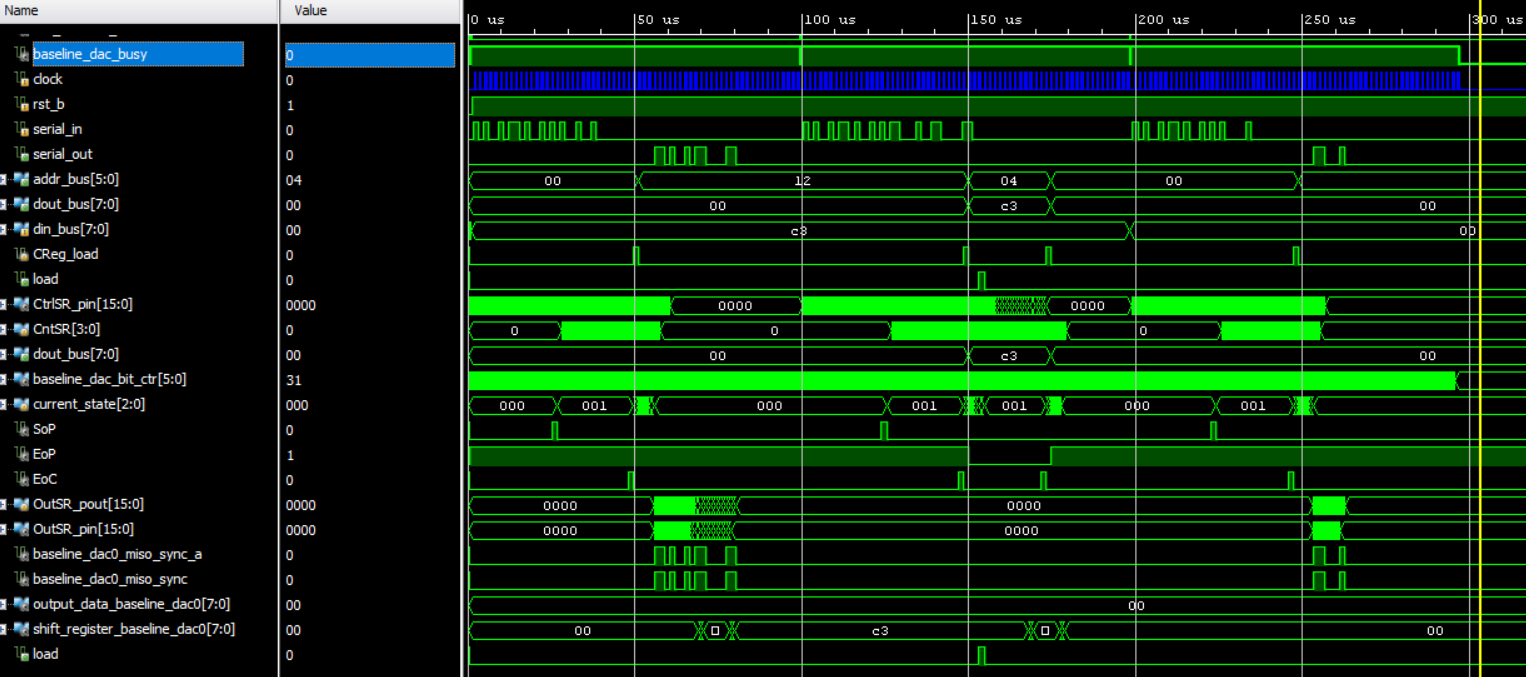
\includegraphics[width=0.85 \textwidth]{IMG/TotalSimulation.png}
		\end{center}
	\end{frame}

	\begin{frame}
	\frametitle{Writing Baseline DACs $\rightarrow$ clock stats}
	\begin{itemize}
		\item clock period of \textbf{98.44} $\mu$s measured with oscilloscope
		\item the signal amplitude is reduced to \textbf{1.2}V from \textbf{2.5}V with a resistive voltage divider 
	\end{itemize}
	\begin{center}
		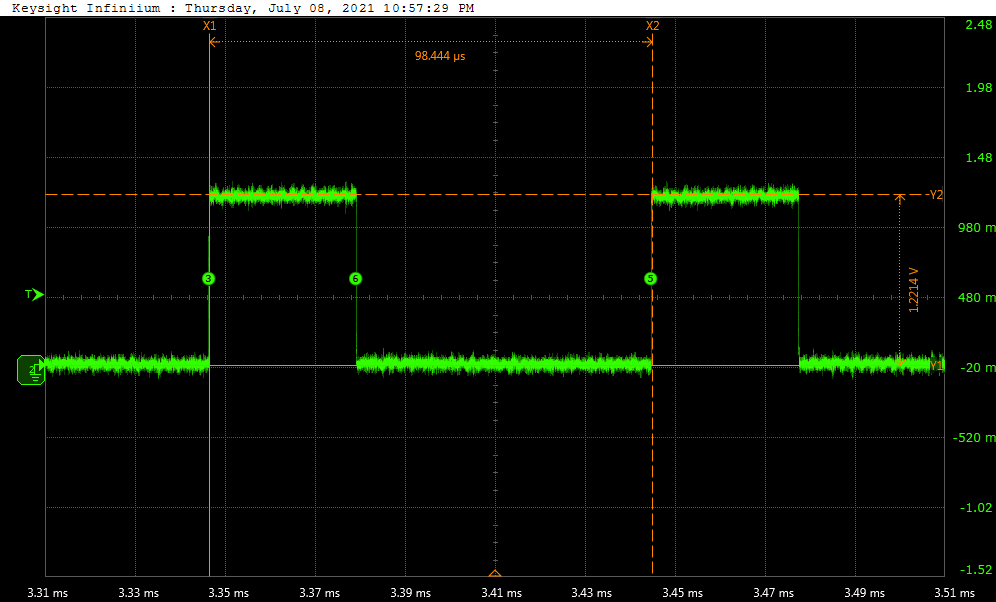
\includegraphics[width=0.65 \textwidth]{IMG/probe/09-08-2021_clock-specks.png}
	\end{center}
	\end{frame}

	\begin{frame}
	\frametitle{Writing Baseline DACs $\rightarrow$ clock stats}
	\begin{itemize}
		\item \textbf{6.29}ms / \textbf{98.44}  $\mu$s $\approx$ \textbf{64} = Number of clock in a data packet
		\item \textbf{32} clock periods for the data transmission + \textbf{32} clock periods waiting for a response
		
	\end{itemize}
	\begin{center}
		\begin{figure}
			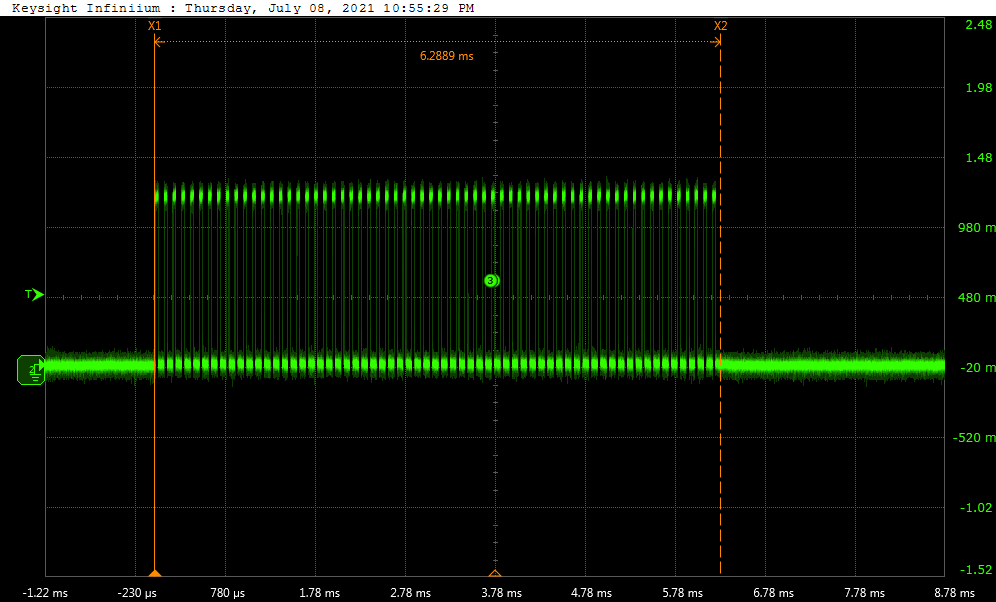
\includegraphics[width=0.65 \textwidth]{IMG/probe/09-08-2021_packet-time.png}
		\end{figure}	
	\end{center}
	\end{frame}

	\begin{frame}
	\frametitle{Writing Baseline DACs $\rightarrow$ data}
	\begin{itemize}
		\item writing sequence for channels \textbf{05} and \textbf{17}
	\end{itemize}
	\begin{columns}
		\column{0.50 \textwidth}
		\begin{center}
			\begin{figure}
				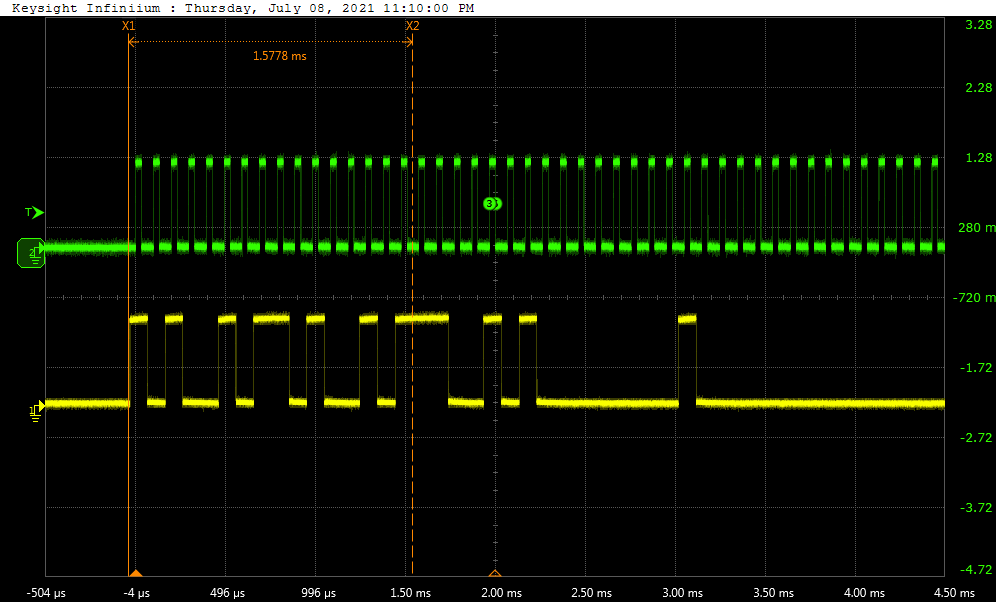
\includegraphics[width=0.55 \textwidth]{IMG/probe/09-08-2021_ch05-write01-baselinedac1.png}
				\caption{\centering{\tiny 11-001010-00000001 ch05-write01}}
			\end{figure}
			\begin{figure}
				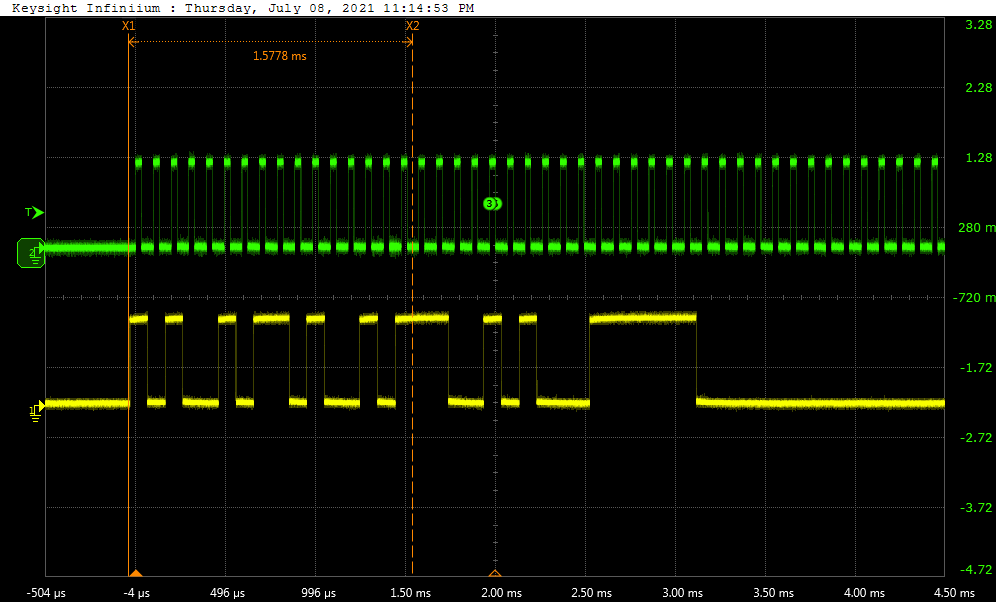
\includegraphics[width=0.55 \textwidth]{IMG/probe/09-08-2021_ch05-write63-baselinedac1.png}
				\caption{\centering{\tiny 11-001010-00111111 ch05-write63}}
			\end{figure}		
		\end{center}
		\column{0.50 \textwidth}
		
		\begin{center}
			\begin{figure}
				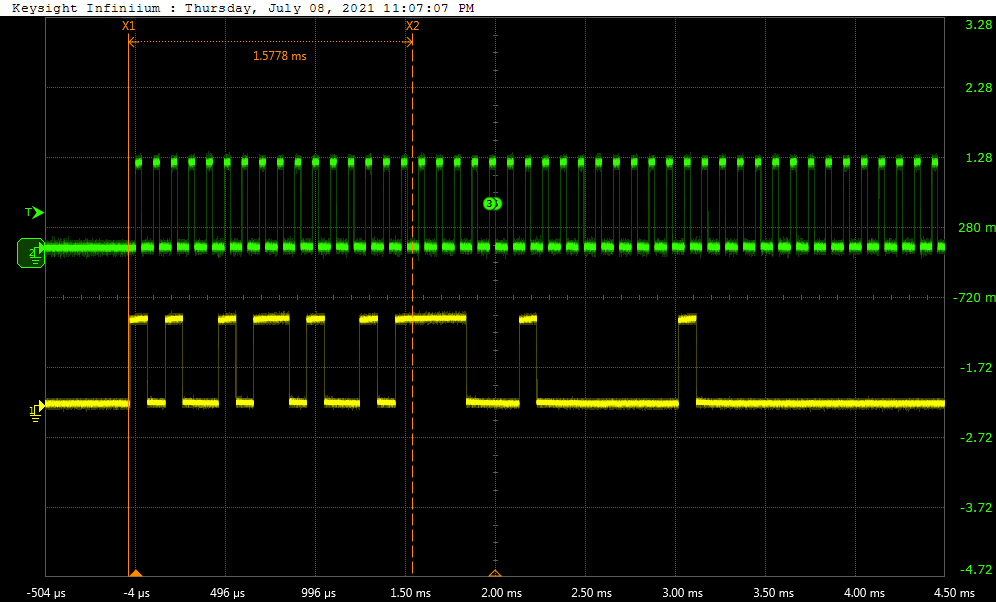
\includegraphics[width=0.55 \textwidth]{IMG/probe/09-08-2021_ch17-write01-baselinedac1.png}
				\caption{\centering{\tiny 11-100010-00000001 ch17-write01}}
			\end{figure}
			\begin{figure}
				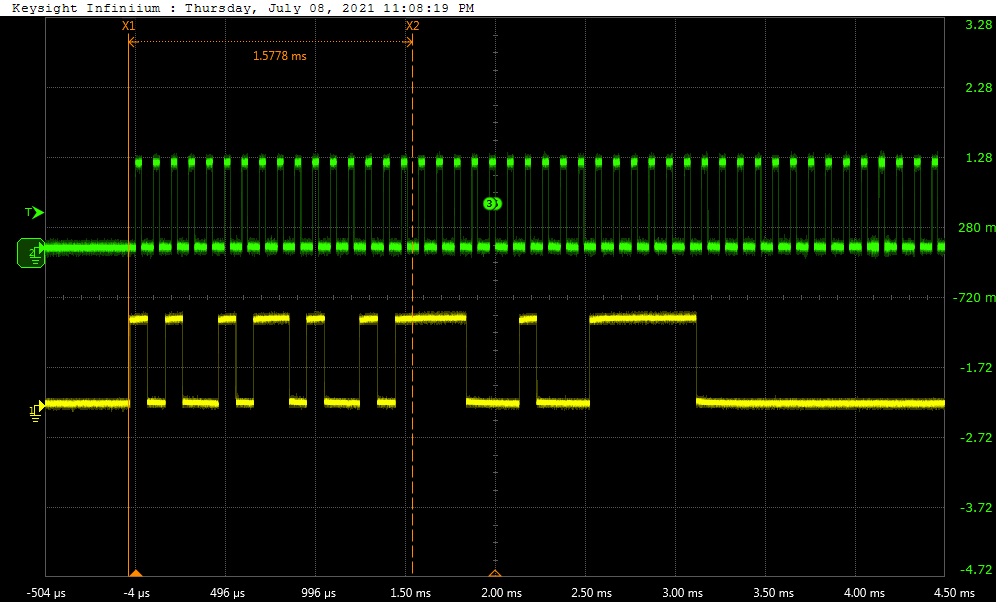
\includegraphics[width=0.55 \textwidth]{IMG/probe/09-08-2021_ch17-write63-baselinedac1.png}
				\caption{\centering{\tiny 11-100010-00111111 ch17-write63}}
			\end{figure}	
		\end{center}
	\end{columns}
	\end{frame}

	\begin{frame}
	\frametitle{Reading Baseline DACs $\rightarrow$ code}
	\begin{itemize}
		\item \textbf{reading} procedure for 1 dac consist of \textbf{2 processes}=
		\begin{itemize}
			\item \textbf{16}bit shift register
			\item sequence detector 
		\end{itemize}
	\end{itemize}
		\begin{center}
			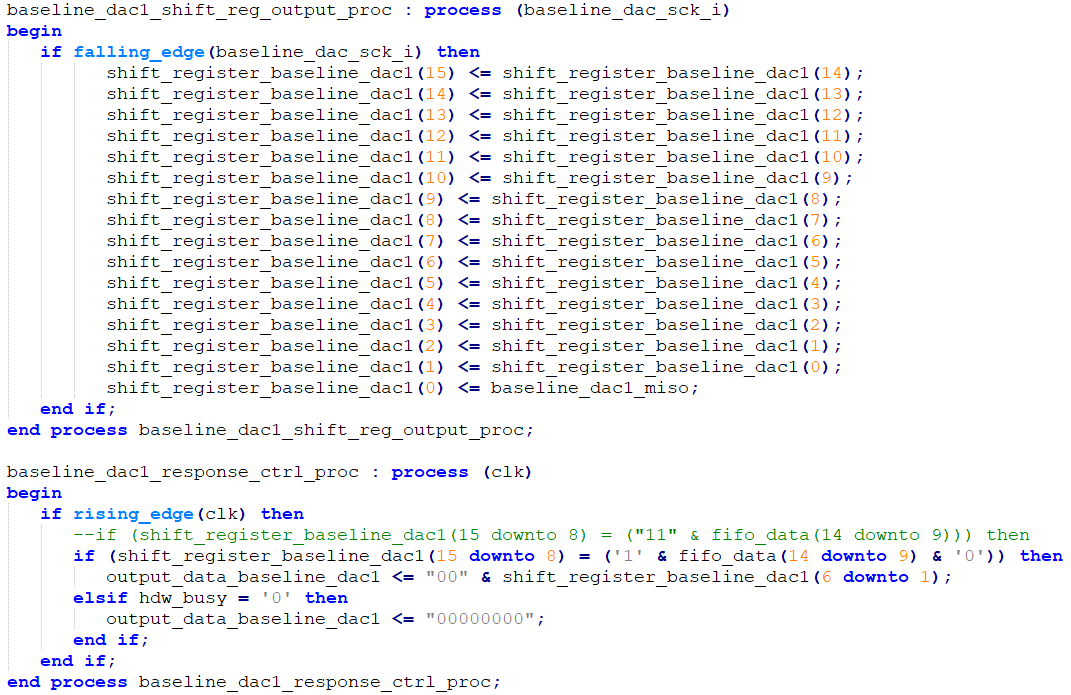
\includegraphics[width=0.6 \textwidth]{IMG/FSM_Read_States.png}
		\end{center}
	\end{frame}

	\begin{frame}
	\frametitle{Level translator}
	\begin{columns}
		\column{0.35 \textwidth}
		\begin{center}
			\begin{figure}
				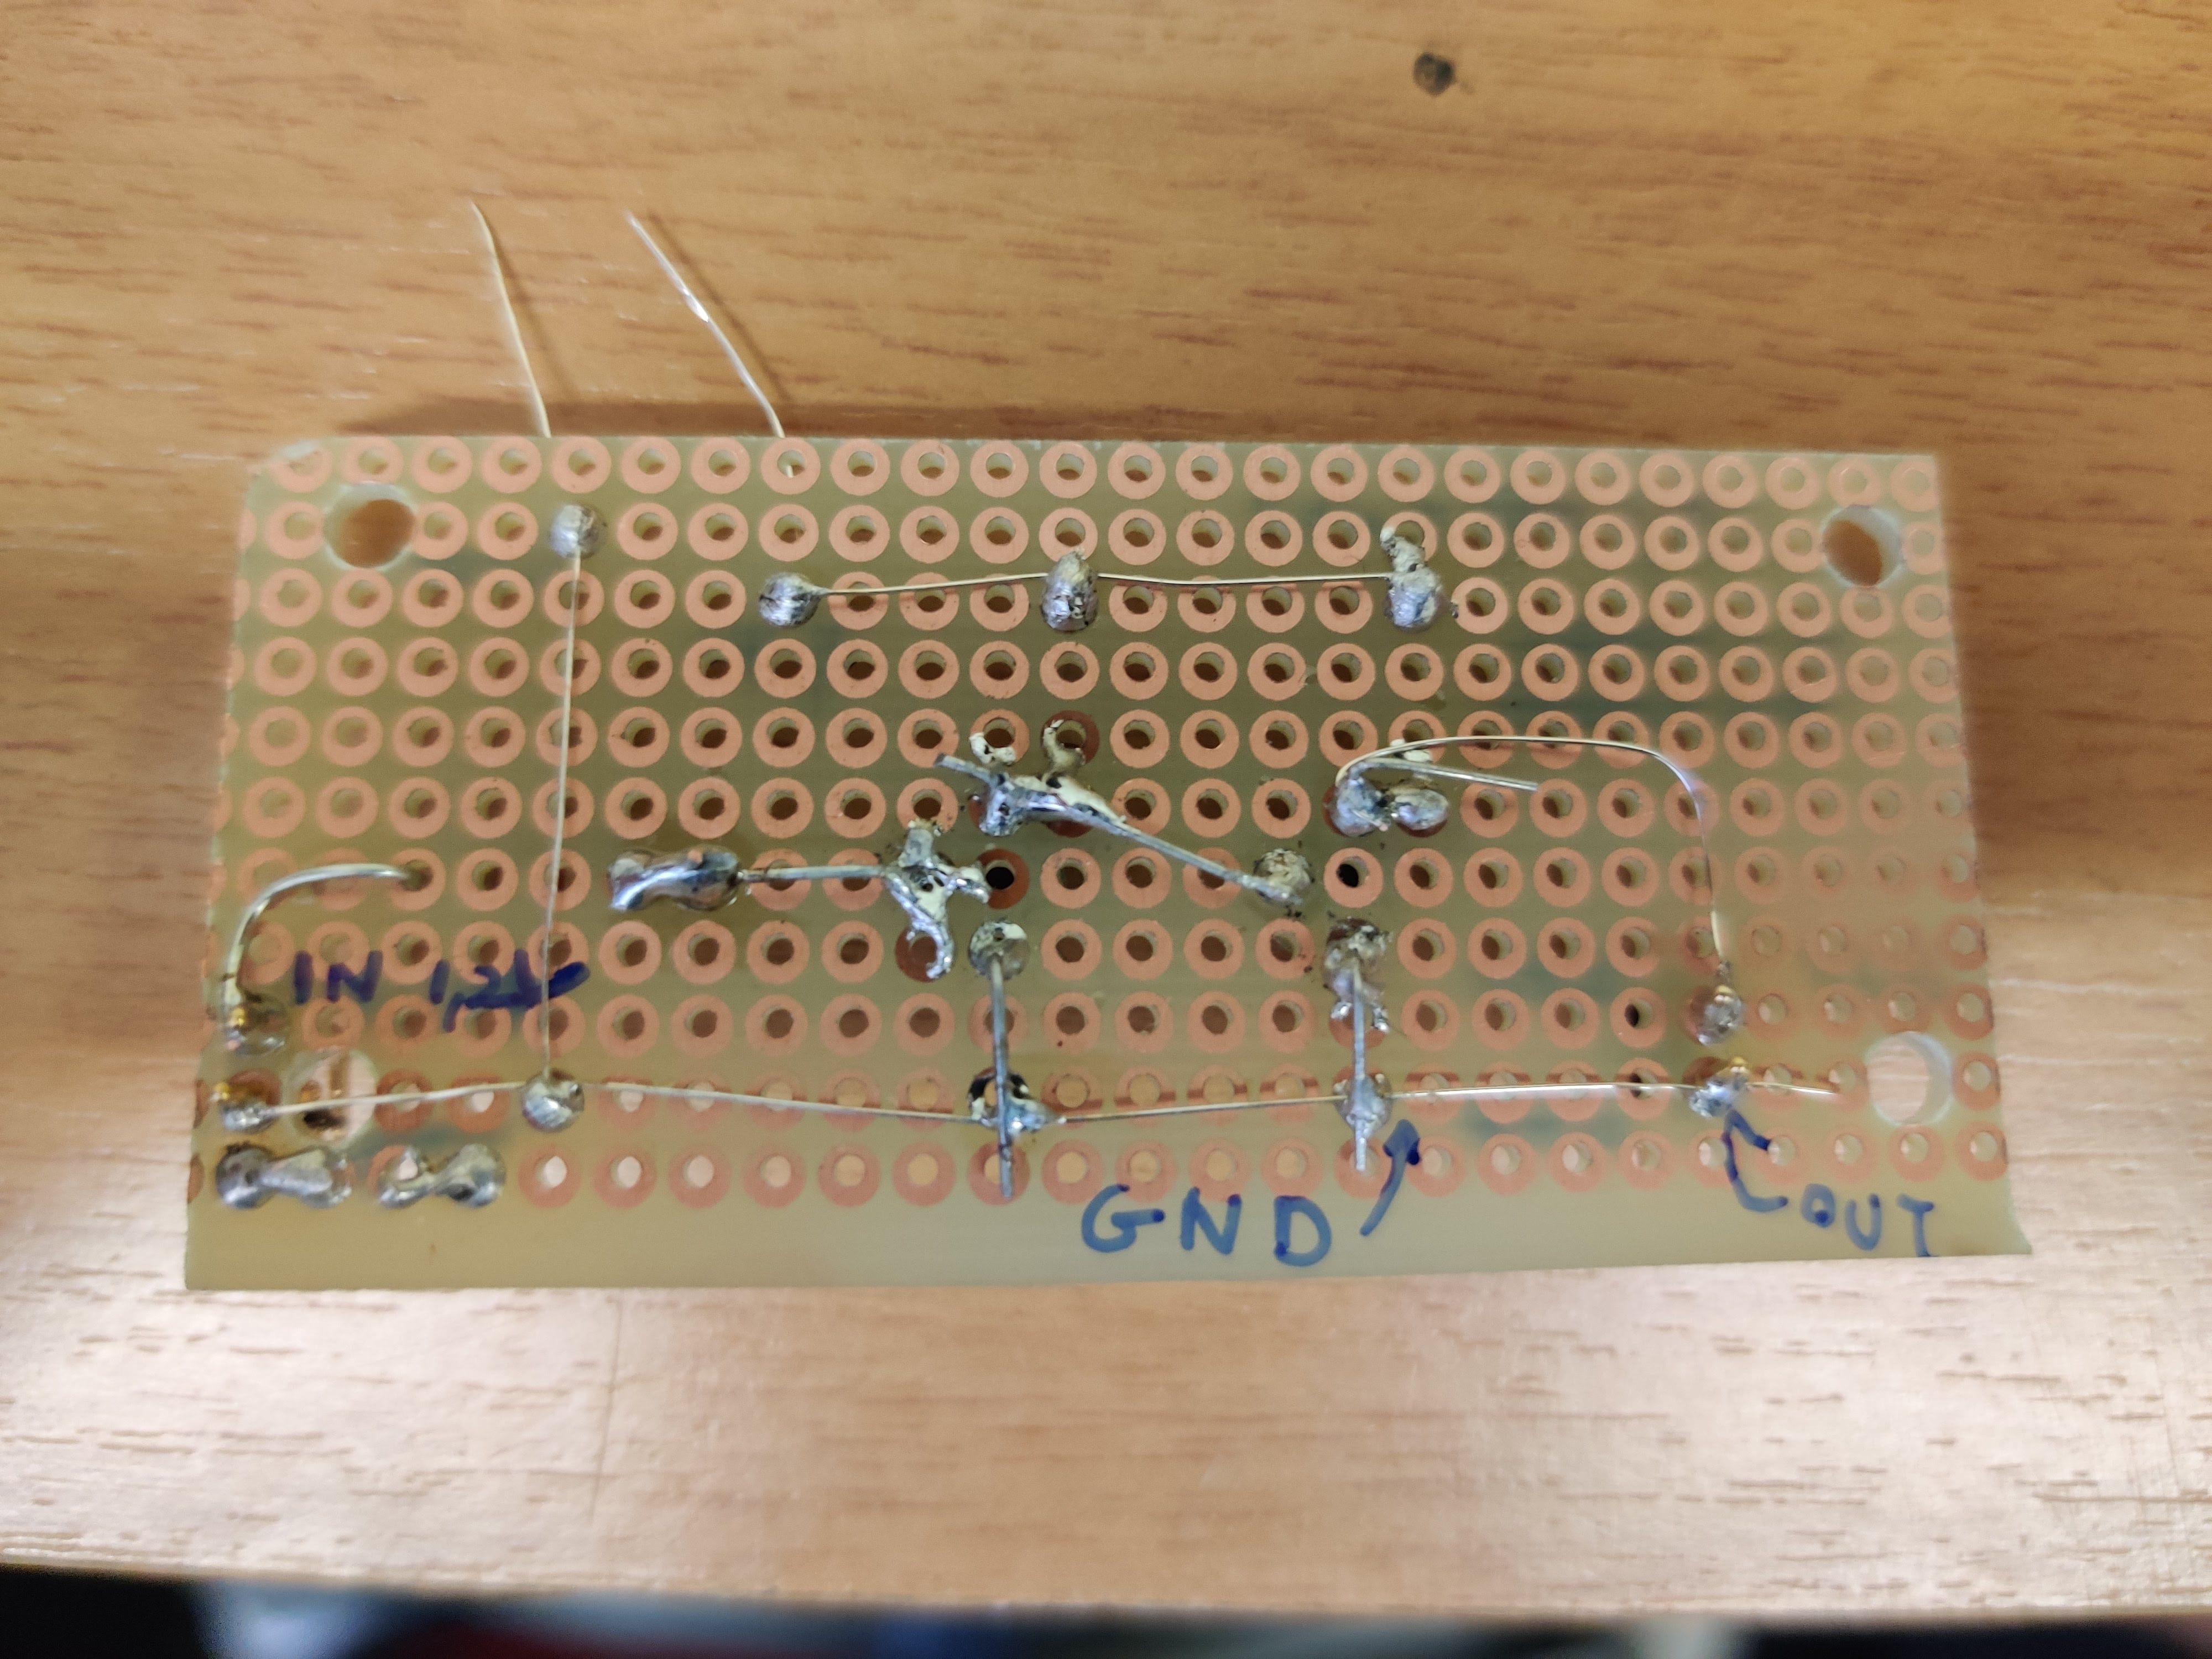
\includegraphics[width=0.8 \textwidth]{IMG/level_translator_back-min.jpg}
			\end{figure}
			\begin{figure}
				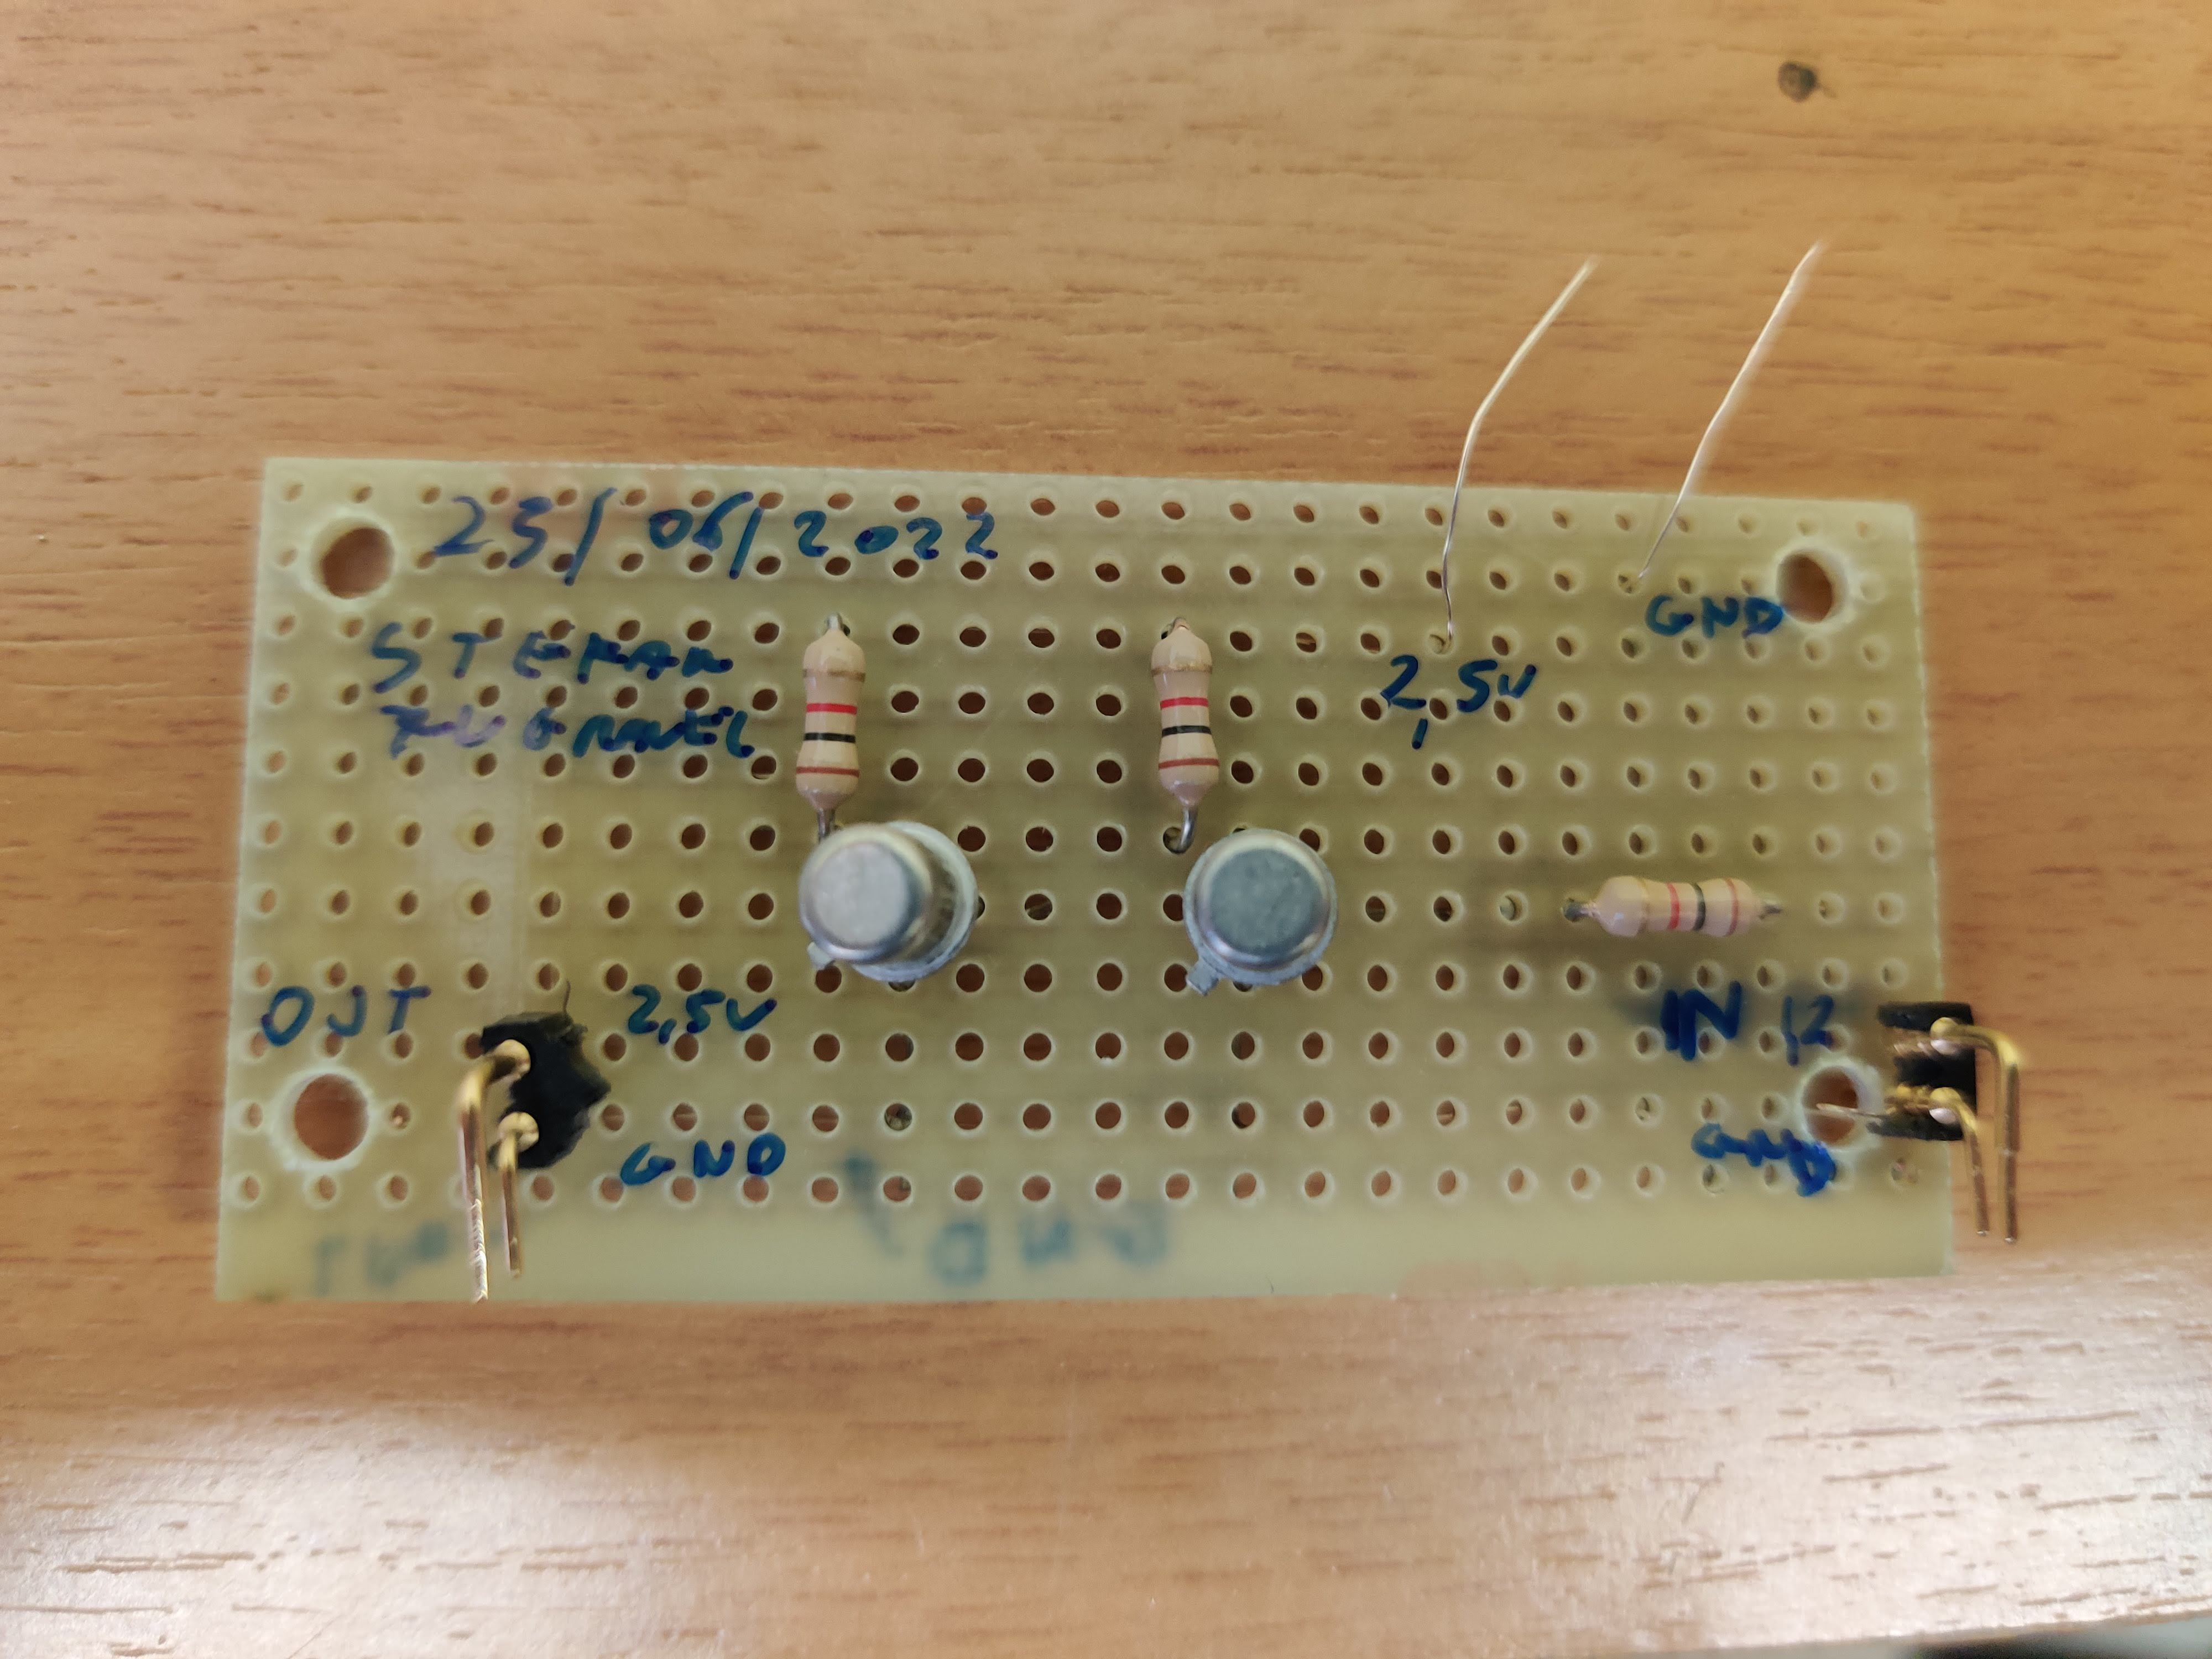
\includegraphics[width=0.8 \textwidth]{IMG/level_translator_front-min.jpg}
			\end{figure}
		\end{center}
		\column{0.65 \textwidth}
		\begin{itemize}
			\item ABACUS output = \textbf{1.2}V single-ended
			\item FPGA input = \textbf{2.5}V single-ended
			\item 2x \textbf{2N2222} NPN transistor in TO-18 package
			\item 3x \textbf{1}k$\Omega$ resistor 1/8W
			\item 2x connectors \& wire
		\end{itemize}
		\begin{figure}
			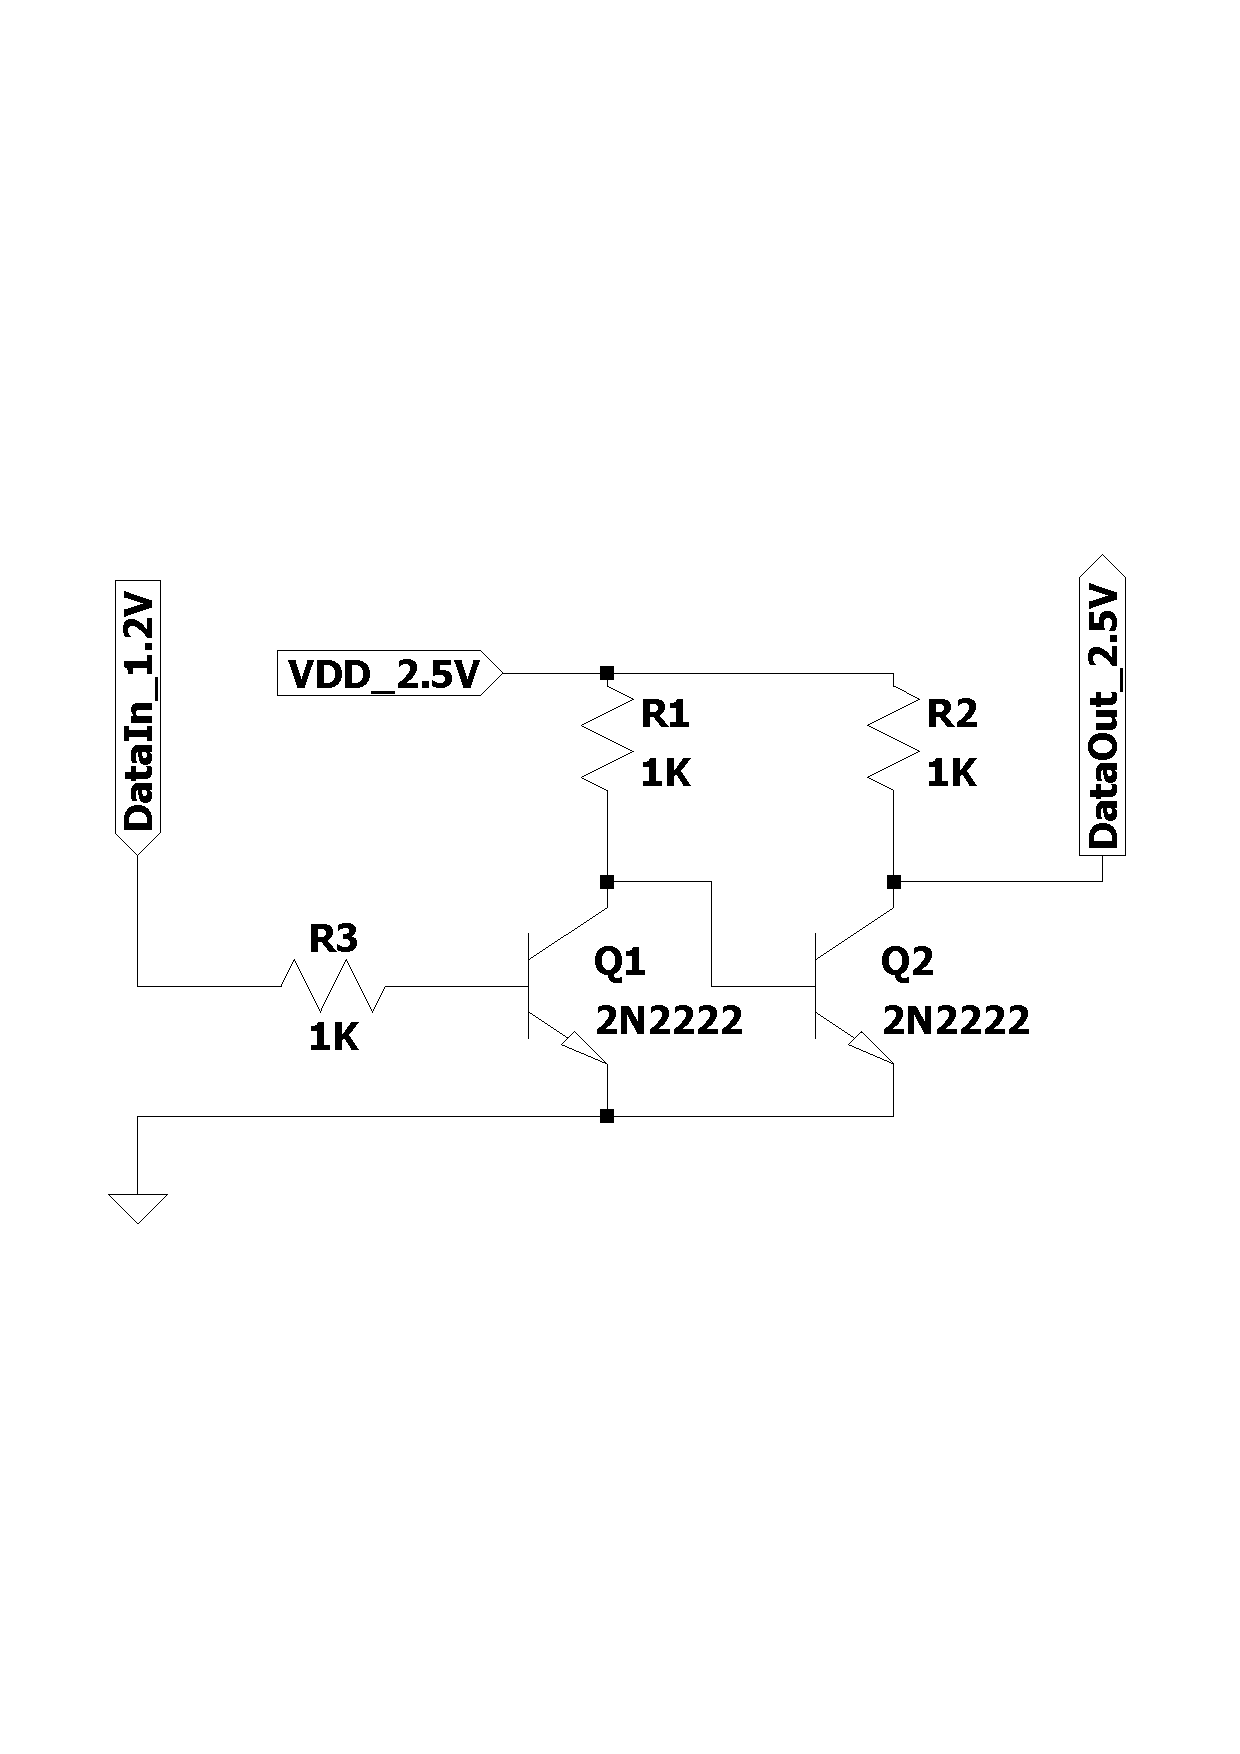
\includegraphics[width=0.6 \textwidth]{IMG/Diagram_cropped.pdf}
		\end{figure}
	\end{columns}
				
	
	
	\end{frame}

	\begin{frame}
	\frametitle{Reading Baseline DACs $\rightarrow$ data}
	\begin{itemize}
		\item reading sequence for channels \textbf{05} and \textbf{07}
	\end{itemize}
	\begin{columns}
		\column{0.50 \textwidth}
		\begin{center}
			\begin{figure}
				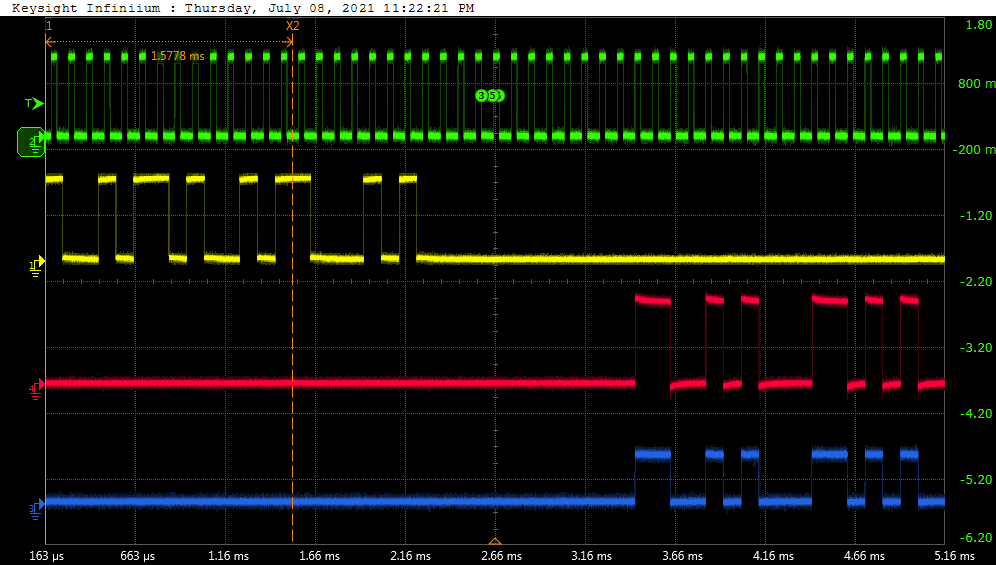
\includegraphics[width=0.55 \textwidth]{IMG/probe/09-08-2021_ch05-read53-baselinedac1.png}
				\caption{\centering{\tiny 10-001010-00000000 ch05-read53}}
			\end{figure}
			\begin{figure}
				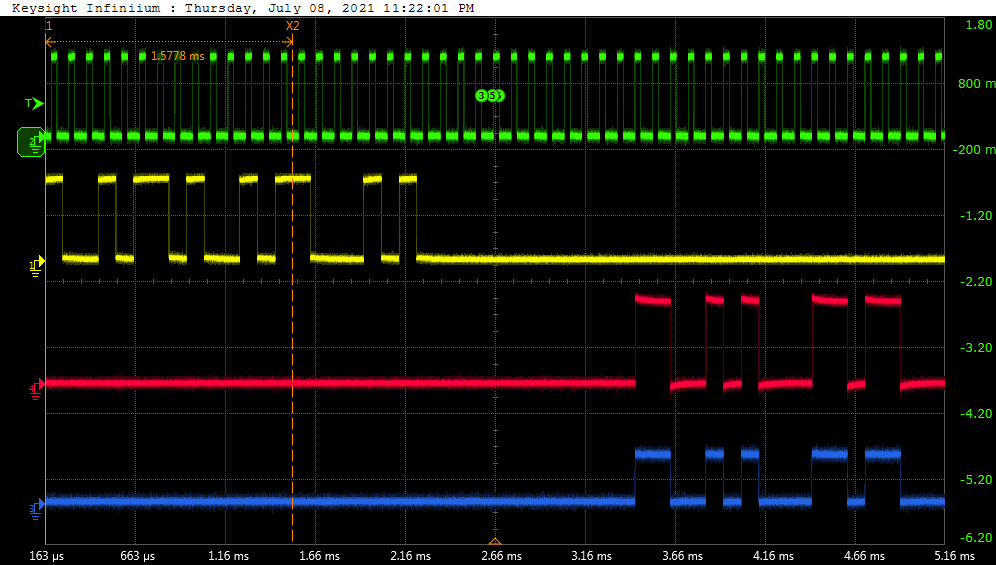
\includegraphics[width=0.55 \textwidth]{IMG/probe/09-08-2021_ch05-read54-baselinedac1.png}
				\caption{\centering{\tiny 10-001010-00000000 ch05-read54}}
			\end{figure}		
		\end{center}
		\column{0.50 \textwidth}
		
		\begin{center}
			\begin{figure}
				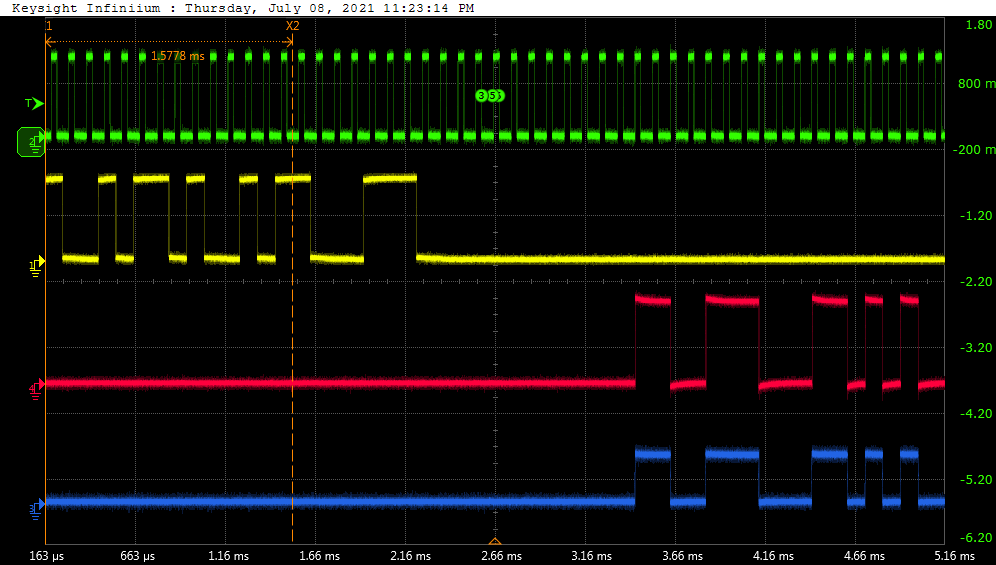
\includegraphics[width=0.55 \textwidth]{IMG/probe/09-08-2021_ch07-read53-baselinedac1.png}
				\caption{\centering{\tiny 10-001110-00000000 ch07-read53}}
			\end{figure}
			\begin{figure}
				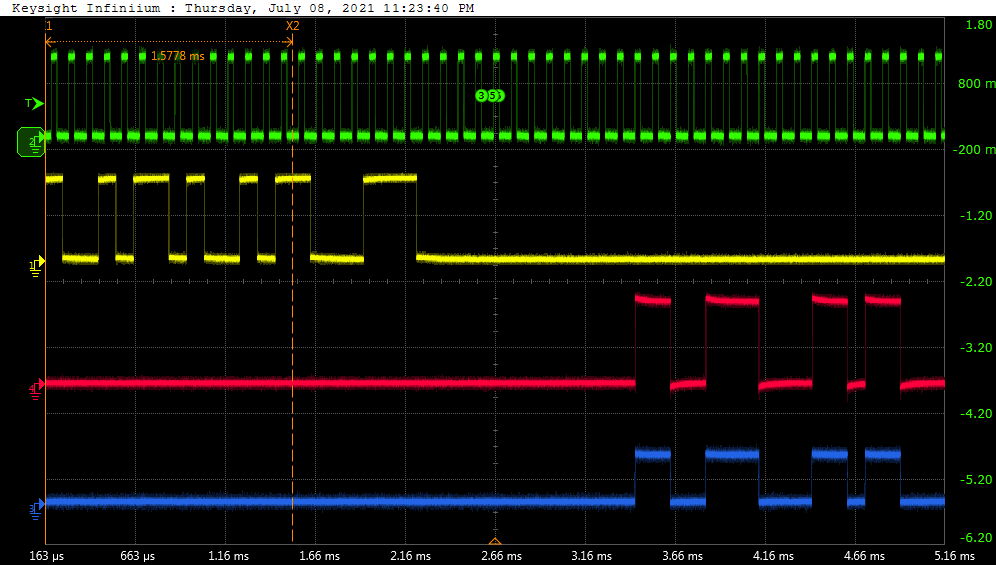
\includegraphics[width=0.55 \textwidth]{IMG/probe/09-08-2021_ch07-read54-baselinedac1.png}
				\caption{\centering{\tiny 10-001110-00000000 ch07-read54}}
			\end{figure}	
		\end{center}
	\end{columns}
	\end{frame}

%%%%%%%%%%%%%%%%%%%%%%%%%%%%%%%%%%%%%%%%%%%%%%%%%%%%%%%%%%%%%%%%%%%%%%%%%%%%%%%%%%%%%%%%
	\section{Constraints}
	
	\begin{frame}[fragile]
	\frametitle{Constraints}
	\begin{itemize}
		\item single-ended constraints \textbf{LVCMOS25} = \textbf{L}ow \textbf{V}oltage \textbf{C}omplementary \textbf{M}etal \textbf{O}xide \textbf{S}emiconductor $\bf{2.5 \pm 0.2}$V
		\item LVCMOS25 $\neq $ LVDS25
	\end{itemize}
	{\tiny 
		\begin{verbatim}
			##Single-ended signal for baseline dac1#######################################
			# FMC_HPC_LA01_CC_P
			set_property -dict { PACKAGE_PIN D26	IOSTANDARD LVCMOS25 DIFF_TERM TRUE}	[get_ports baseline_dac1_sck]
			# FMC_HPC_LA01_CC_N
			set_property -dict { PACKAGE_PIN C26	IOSTANDARD LVCMOS25 DIFF_TERM TRUE}	[get_ports gnd_10]
			#
			# FMC_HPC_LA06_P
			set_property -dict { PACKAGE_PIN H30	IOSTANDARD LVCMOS25 DIFF_TERM TRUE}	[get_ports baseline_dac1_mosi]
			# FMC_HPC_LA06_N
			set_property -dict { PACKAGE_PIN G30	IOSTANDARD LVCMOS25 DIFF_TERM TRUE}	[get_ports gnd_11]
			#
			# FMC_HPC_LA05_P
			set_property -dict { PACKAGE_PIN G29	IOSTANDARD LVCMOS25 DIFF_TERM TRUE}	[get_ports baseline_dac1_miso]
			# FMC_HPC_LA05_N
			set_property -dict { PACKAGE_PIN F30	IOSTANDARD LVCMOS25 DIFF_TERM TRUE}	[get_ports gnd_12]
				
		\end{verbatim} 
						}
	\end{frame}

%%%%%%%%%%%%%%%%%%%%%%%%%%%%%%%%%%%%%%%%%%%%%%%%%%%%%%%%%%%%%%%%%%%%%%%%%%%%%%%%%%%%%%%%
	\section{Results}
	
	\begin{frame}
	\frametitle{results}
	\begin{center}
		{\Huge \fontfamily{qtm}\selectfont \color{blue} \textbf{Results}}
	\end{center}
	\end{frame}
	
	\begin{frame}
	\frametitle{threshold scan}
		\begin{itemize}
			\item channel 1 threshold scan with \textbf{600}mV \textbf{10}KHz impulses
			\item {\color{blue}blue} curve with baseline dac=\textbf{0}
			\item {\color{green}green} curve with baseline dac=\textbf{63}  
		\end{itemize}	
		\begin{center}
			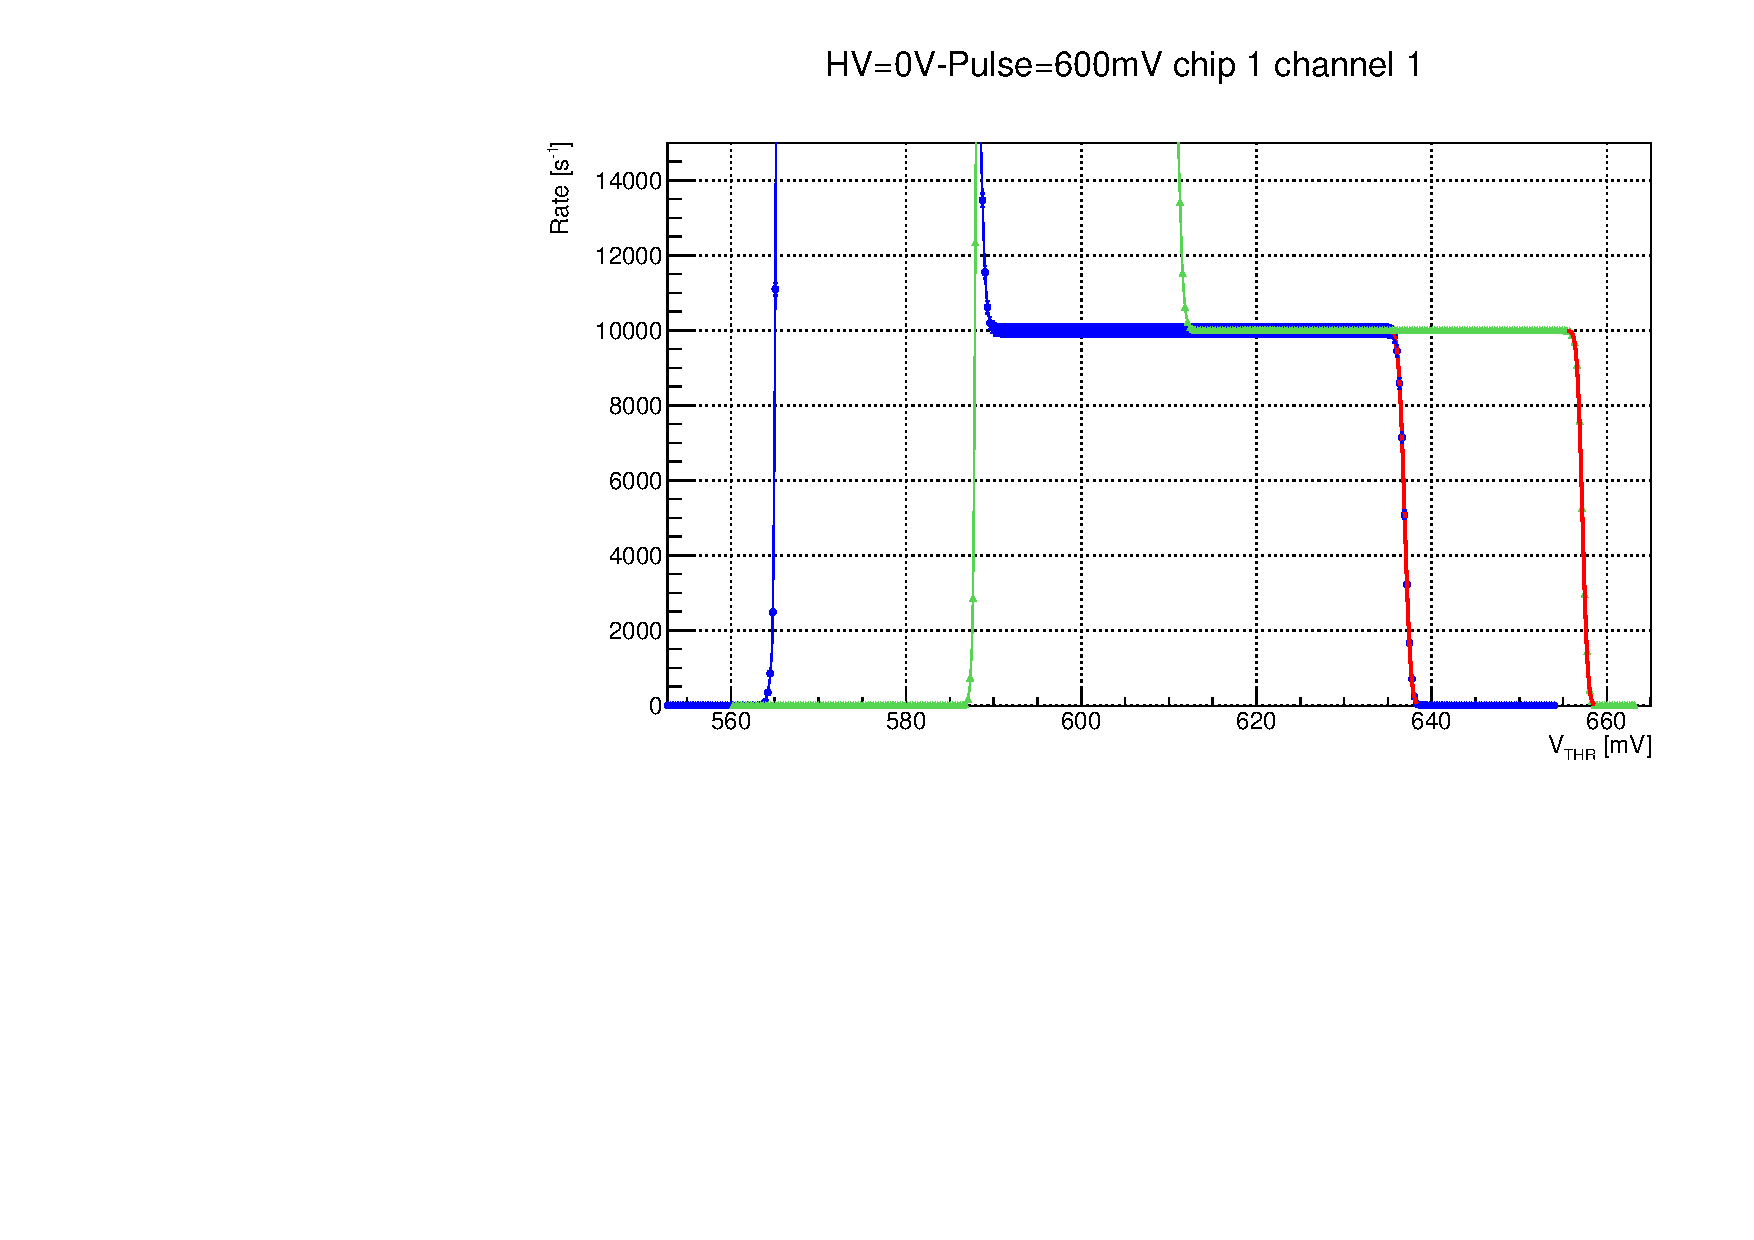
\includegraphics[width=0.65 \textwidth]{IMG/ThScan_ch0.pdf}
		\end{center}
		
	\end{frame}

	\begin{frame}
	\frametitle{Pedestal distribution}
	\begin{itemize}
		\item pedestal voltage value for odd channels
		\item {\color{blue}blue} dots with baseline dac=\textbf{0}
		\item {\color{red}red} dots with baseline dac=\textbf{63}
	\end{itemize}
	\begin{center}
		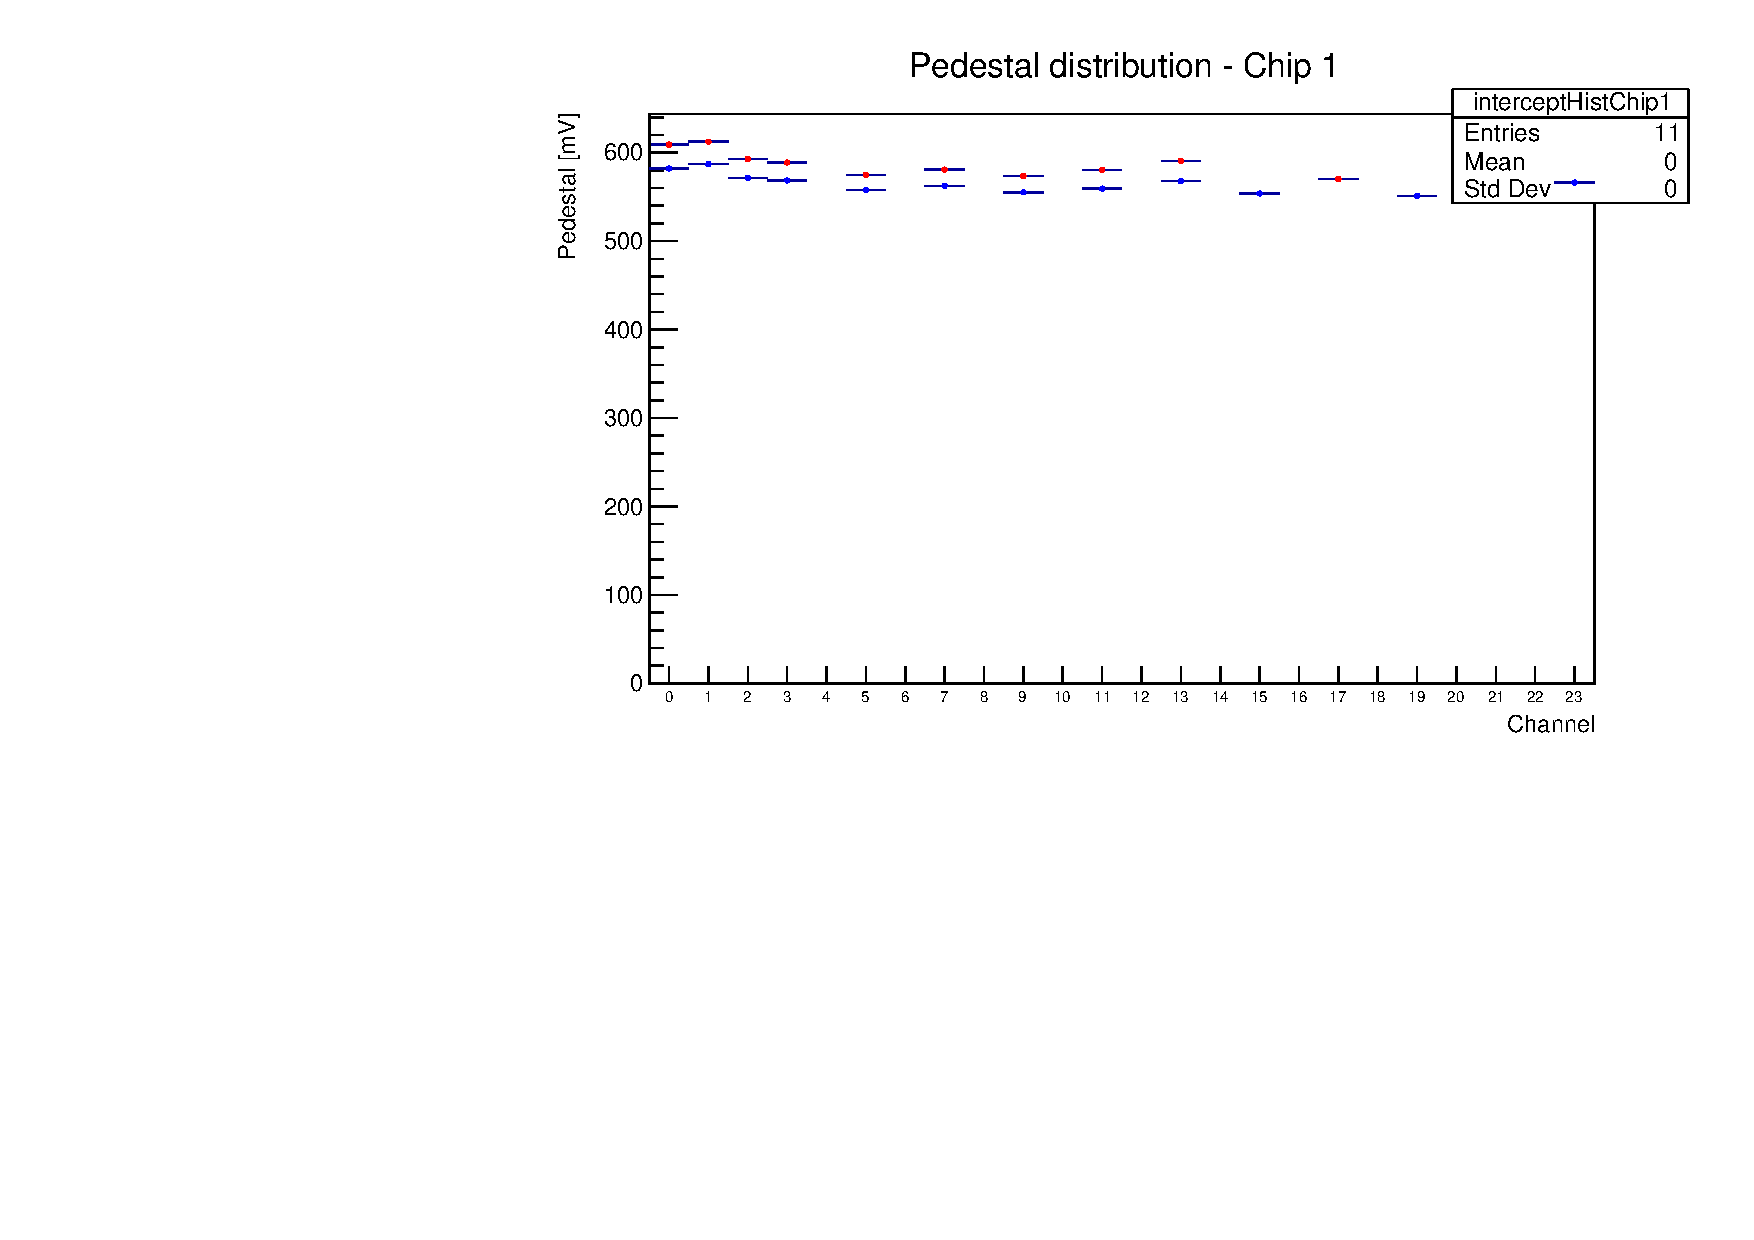
\includegraphics[width=0.65 \textwidth]{IMG/TB1-DAC0-DAC63.pdf}
	\end{center}
	
	\end{frame}

%%%%%%%%%%%%%%%%%%%%%%%%%%%%%%%%%%%%%%%%%%%%%%%%%%%%%%%%%%%%%%%%%%%%%%%%%%%%%%%%%%%%%%%%
	\section{Conclusions}
	
	\begin{frame}
	\frametitle{Conclusions }
	\begin{center}
		\textbf{Future additions to the FPGA firmware}
	\end{center}
		\begin{itemize}
			\item addition of a \textbf{latch} in order to save into a \textbf{register} the current state of every counter 
			\item addition of a \textbf{timestamp} in order to obtain a more accurate rate calculation 
			\item addition of a configurable \textbf{mask} to calculate via firmware the \textbf{sum} of only certain selected channels 
			
		\end{itemize}
	
	\vspace{1 cm}
		\begin{center}
			\textbf{Thanks for the attention!!}
		\end{center}
		
	\end{frame}

	\begin{frame}
	\frametitle{Bibliography}
	{\scriptsize 
	\begin{thebibliography}{00}
		\bibitem{1}www.researchgate.net/figure/Dose-depth-curve-for-monoenergetic-photons-protons-and-carbon-ions-courtesy-of-GSI$\textunderscore$fig1$\textunderscore$283521369
		\newline
		\bibitem{2}www.intechopen.com/books/novel-prospects-in-oxidative-and-nitrosative-stress/oxidative-stress-in-hadrontherapy
		\newline
		\bibitem{3}www.semanticscholar.org/paper/A-Millimeter-Scale-Single-Charged-Particle-for-Lee-Scholey/ae955a07a42e9c124a8473357cd485b0b9928090
		\newline
		\bibitem{4}www.semanticscholar.org/paper/Low-Gain-Avalanche-Detectors-(LGAD)-for-particle-Moffat-Bates/0477d7bc2c9a3b26ad776874598f56d7d5b54c45
		\newline
		\bibitem{5}MoveIt v2 design document, Giovanni Mazza, January 15, 2021
	\end{thebibliography} }
	\end{frame}

%%%%%%%%%%%%%%%%%%%%%%%%%%%%%%%%%%%%%%%%%%%%%%%%%%%%%%%%%%%%%%%%%%%%%%%%%%%%%%%%%%%%%%%%
	\section{Auxiliary images}
	
	\begin{frame}
	\frametitle{Additional Graphs}
	\begin{columns}
		\column{0.3 \textwidth}
		\begin{center}
			\begin{figure}
				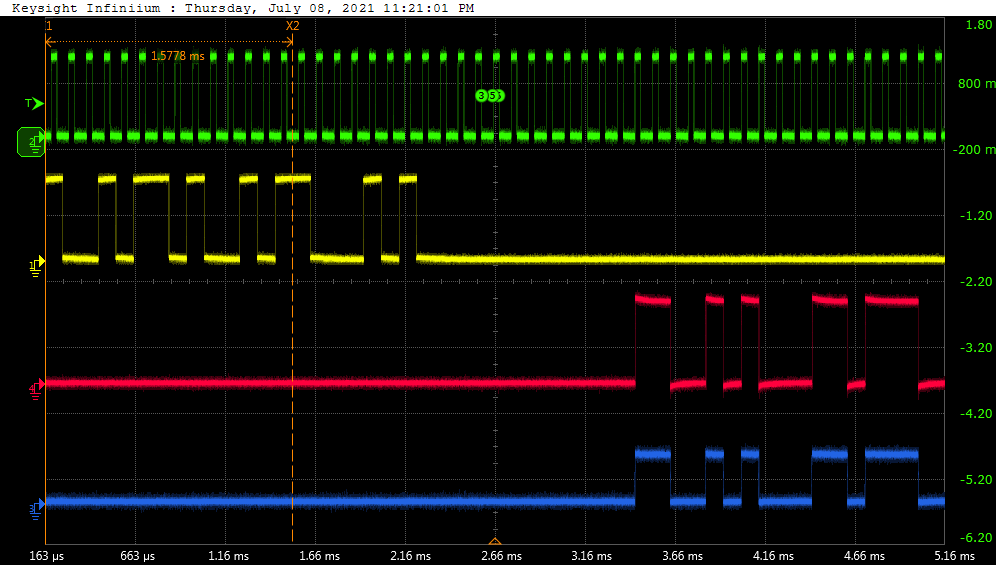
\includegraphics[width=0.95 \textwidth]{IMG/probe/09-08-2021_ch05-read55-baselinedac1.png}
				\caption{\centering{\tiny ch05-read55}}
			\end{figure}
			\begin{figure}
				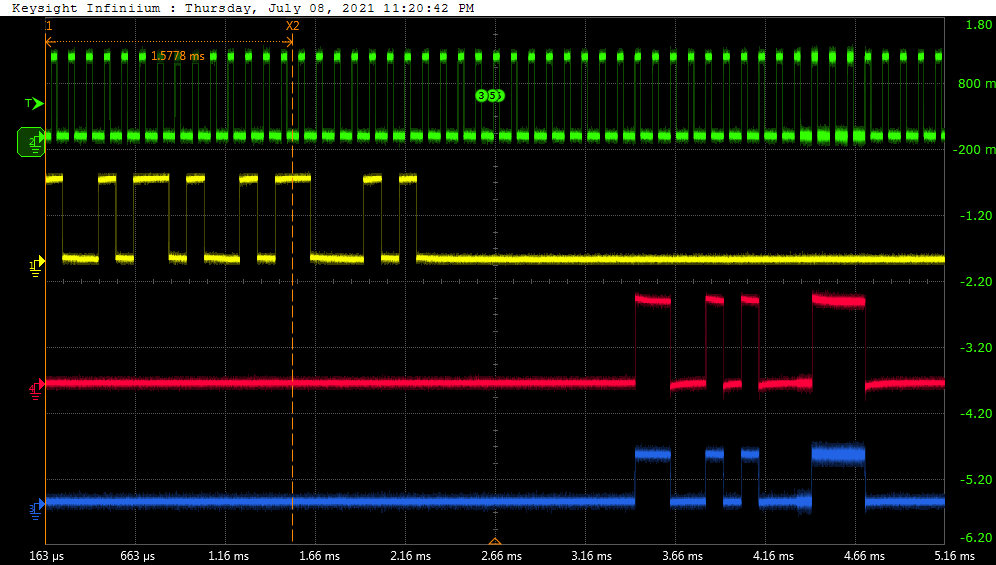
\includegraphics[width=0.95 \textwidth]{IMG/probe/09-08-2021_ch05-read56-baselinedac1.png}
				\caption{\centering{\tiny ch05-read56}}
			\end{figure}		
		\end{center}
		\column{0.3 \textwidth}
		\begin{center}
			\begin{figure}
				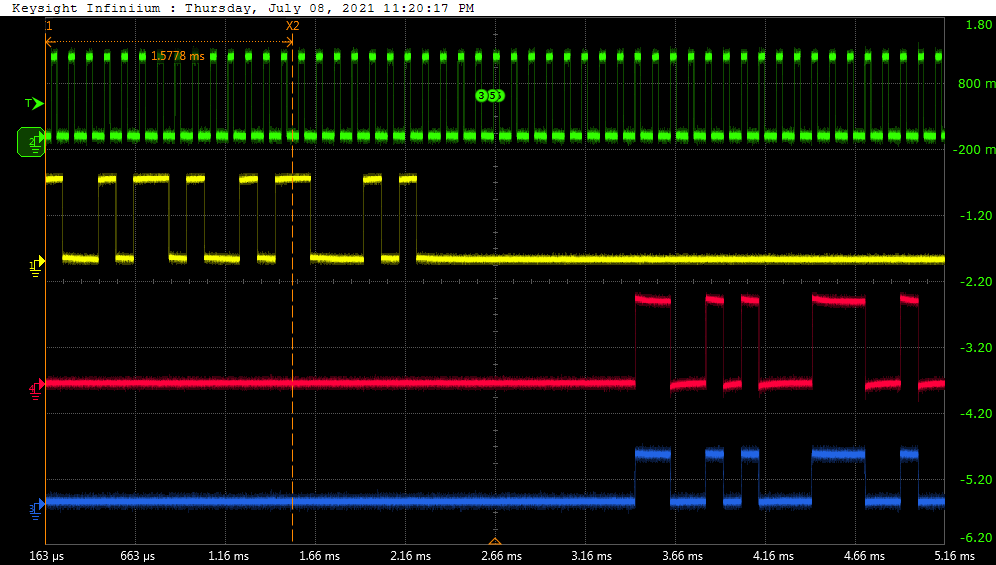
\includegraphics[width=0.95 \textwidth]{IMG/probe/09-08-2021_ch05-read57-baselinedac1.png}
				\caption{\centering{\tiny ch07-read57}}
			\end{figure}
			\begin{figure}
				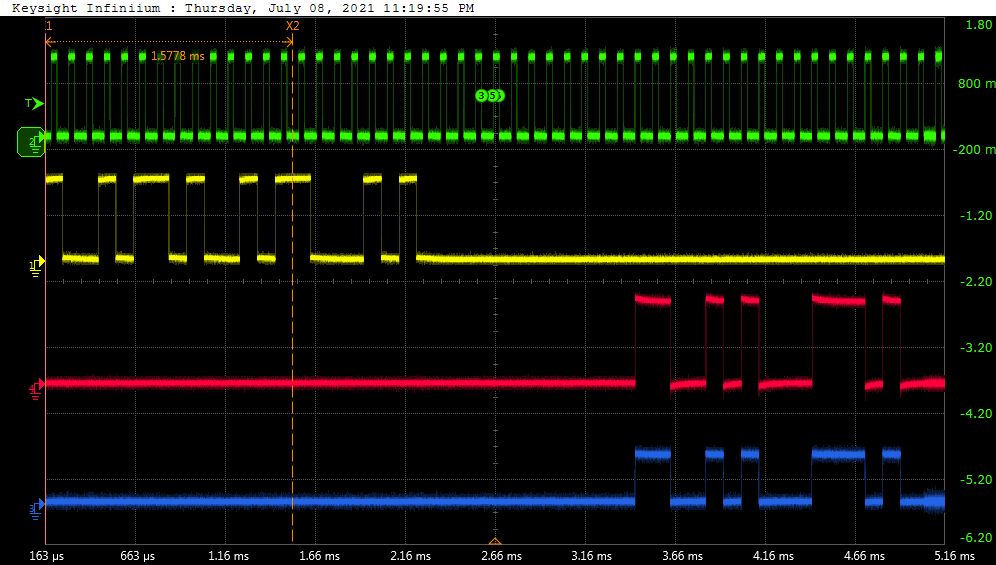
\includegraphics[width=0.95 \textwidth]{IMG/probe/09-08-2021_ch05-read58-baselinedac1.png}
				\caption{\centering{\tiny ch07-read58}}
			\end{figure}	
		\end{center}
		\column{0.3 \textwidth}
		\begin{center}
			\begin{figure}
				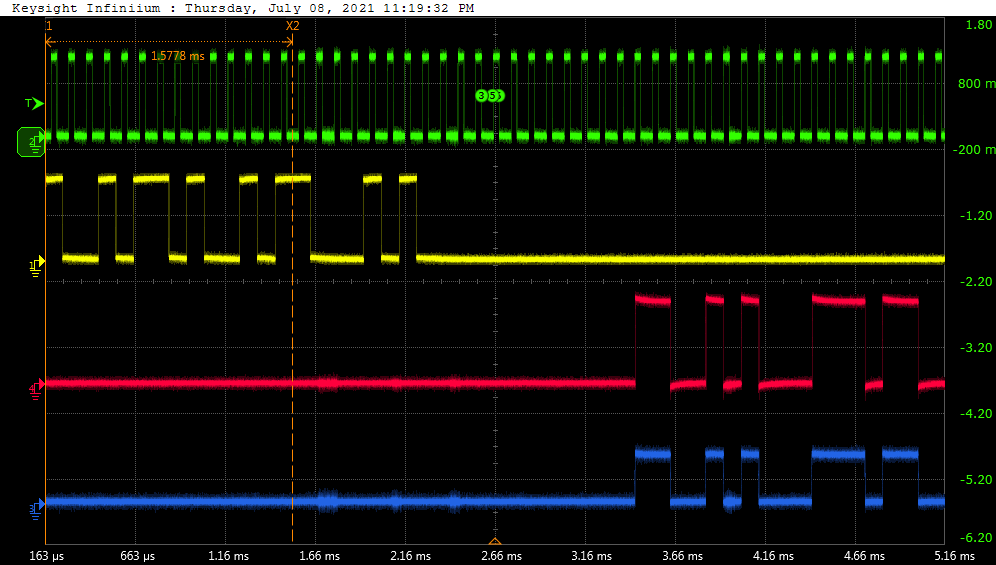
\includegraphics[width=0.95 \textwidth]{IMG/probe/09-08-2021_ch05-read59-baselinedac1.png}
				\caption{\centering{\tiny ch07-read59}}
			\end{figure}
			\begin{figure}
				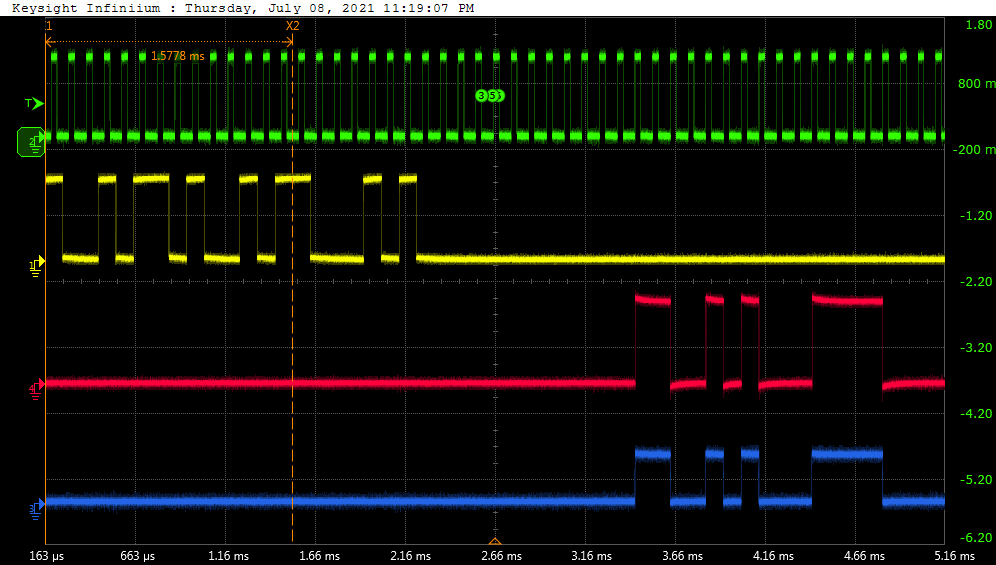
\includegraphics[width=0.95 \textwidth]{IMG/probe/09-08-2021_ch05-read60-baselinedac1.png}
				\caption{\centering{\tiny ch07-read60}}
			\end{figure}	
		\end{center}
	\end{columns}
		\end{frame}
	
\end{document}